\documentclass[12pt,a4paper]{article}

% --- GÓI TIẾNG VIỆT VÀ ĐỊNH DẠNG TRANG CHUẨN MẪU TRƯỜNG ĐH SƯ PHẠM TP.HCM ---
\usepackage[T5]{fontenc}
\usepackage[utf8]{inputenc}
\usepackage[vietnamese]{babel}
\usepackage{tgtermes} % Phông chữ Times New Roman chuẩn (TeX Gyre Termes) đầy đủ dấu tiếng Việt
\usepackage[top=2.5cm, bottom=2.5cm, left=3.0cm, right=2.0cm]{geometry}
\usepackage{amsmath, amssymb, amsfonts}
\usepackage{graphicx}
\usepackage{subcaption}
\usepackage{booktabs, multirow, array}
\usepackage{float}
\usepackage{xcolor}
\usepackage{fancyhdr}
\usepackage{titlesec}
\usepackage{listings}
\usepackage{setspace}
\usepackage{indentfirst}
\usepackage{tikz}
\usepackage{tocloft}
\usepackage{enumitem}
\usepackage[labelsep=period]{caption} % Định dạng nhãn hình/bảng có dấu chấm ngăn cách: "Hình 2-1."
\usepackage[pdfpagelabels=false, colorlinks=true, linkcolor=black, citecolor=black, urlcolor=blue]{hyperref}

\usetikzlibrary{calc, shapes.geometric, arrows.meta, positioning}

% Thiết lập từ điển ngắt từ trong tài liệu tham khảo
\hyphenation{Mikolov Sutskever Schmidhuber Corrado Representations Classification}

% --- THIẾT LẬP GIÃN DÒNG VÀ THỤT ĐẦU DÒNG CHUẨN TIỂU LUẬN ---
\setstretch{1.3}
\setlength{\parindent}{1.0cm}
\setlength{\parskip}{4pt}

% --- THIẾT LẬP ĐÁNH SỐ TRANG Ở GIỮA TRÊN CÙNG TRÊN MỌI TRANG (NHƯ MẪU) ---
\pagestyle{fancy}
\fancyhf{}
\fancyhead[C]{\thepage}
\renewcommand{\headrulewidth}{0pt}
\renewcommand{\footrulewidth}{0pt}
\setlength{\headheight}{15pt}

% Đồng bộ hoá kiểu trang plain (khi bắt đầu chương mới)
\fancypagestyle{plain}{
    \fancyhf{}
    \fancyhead[C]{\thepage}
    \renewcommand{\headrulewidth}{0pt}
    \renewcommand{\footrulewidth}{0pt}
}

% --- ĐỊNH DẠNG TIÊU ĐỀ THEO MẪU TRƯỜNG ĐH SƯ PHẠM TP.HCM ---
\titleformat{\section}[block]{\centering\large\bfseries}{CHƯƠNG \thesection.}{0.5em}{\MakeUppercase}
\titleformat{\subsection}{\normalfont\normalsize\bfseries}{\thesubsection.}{0.5em}{}
\titleformat{\subsubsection}{\normalfont\normalsize\bfseries}{\thesubsubsection.}{0.5em}{}

\titlespacing*{\section}{0pt}{18pt}{14pt}
\titlespacing*{\subsection}{0pt}{12pt}{6pt}
\titlespacing*{\subsubsection}{0pt}{10pt}{4pt}

% --- ĐỊNH DẠNG TÊN HÌNH ẢNH VÀ BẢNG BIỂU ---
\renewcommand{\figurename}{Hình}
\renewcommand{\tablename}{Bảng}
\counterwithin{figure}{section}
\counterwithin{table}{section}
\renewcommand{\thefigure}{\arabic{section}-\arabic{figure}}
\renewcommand{\thetable}{\arabic{section}-\arabic{table}}

% --- THIẾT LẬP LISTINGS MÃ NGUỒN CÓ KHUNG VIỀN NHƯ PHỤ LỤC MẪU ---
\lstset{
    basicstyle=\ttfamily\footnotesize,
    breaklines=true,
    frame=single,
    keepspaces=true,
    numbers=none,
    showspaces=false,
    showstringspaces=false,
    showtabs=false,
    tabsize=2,
    backgroundcolor=\color{white}
}

\begin{document}

% ==============================================================================
% TRANG BÌA CHÍNH (COVER PAGE) - CHUẨN MẪU TRƯỜNG ĐẠI HỌC SƯ PHẠM TP.HCM
% ==============================================================================
\begin{titlepage}
    % Khung đôi viền kèm góc vuông chuẩn tiểu luận trường ĐHSP TP.HCM
    \begin{tikzpicture}[remember picture, overlay]
        % Viền ngoài đậm 2.5pt
        \draw[line width=2.5pt] 
            ($(current page.north west) + (2.0cm, -1.5cm)$) 
            rectangle 
            ($(current page.south east) + (-1.5cm, 1.5cm)$);
        % Viền trong mảnh 0.8pt
        \draw[line width=0.8pt] 
            ($(current page.north west) + (2.16cm, -1.66cm)$) 
            rectangle 
            ($(current page.south east) + (-1.66cm, 1.66cm)$);
        % 4 góc vuông trang trí kinh điển
        \draw[line width=1.0pt] ($(current page.north west) + (2.0cm, -1.5cm)$) ++(0, -0.45cm) -- ++(0.45cm, 0) -- ++(0, 0.45cm);
        \draw[line width=1.0pt] ($(current page.north east) + (-1.5cm, -1.5cm)$) ++(0, -0.45cm) -- ++(-0.45cm, 0) -- ++(0, 0.45cm);
        \draw[line width=1.0pt] ($(current page.south west) + (2.0cm, 1.5cm)$) ++(0, 0.45cm) -- ++(0.45cm, 0) -- ++(0, -0.45cm);
        \draw[line width=1.0pt] ($(current page.south east) + (-1.5cm, 1.5cm)$) ++(0, 0.45cm) -- ++(-0.45cm, 0) -- ++(0, -0.45cm);
    \end{tikzpicture}

    \begin{center}
        {\large\bfseries BỘ GIÁO DỤC VÀ ĐÀO TẠO}\\[0.2cm]
        {\large\bfseries TRƯỜNG ĐẠI HỌC SƯ PHẠM THÀNH PHỐ HỒ CHÍ MINH}\\[1.0cm]

        % Bảng điểm thi chuẩn mẫu
        \renewcommand{\arraystretch}{1.3}
        \begin{tabular}{|m{2.1cm}|m{2.3cm}|m{4.8cm}|m{4.8cm}|}
            \hline
            \centering\bfseries ĐIỂM SỐ & \centering\bfseries ĐIỂM CHỮ & \centering\bfseries Cán bộ chấm thi 1\par\small (Ký, ghi rõ họ tên) & \centering\arraybackslash\bfseries Cán bộ chấm thi 2\par\small (Ký, ghi rõ họ tên) \\
            \hline
            \rule{0pt}{1.8cm} & & & \\[1.8cm]
            \hline
        \end{tabular}

        \vspace{1.3cm}

        % Tên đề tài (Trực tiếp tiêu đề in hoa đậm căn đều như mẫu)
        {\Large\bfseries TÌM HIỂU CÁC PHƯƠNG PHÁP WORD2VEC,}\\[0.25cm]
        {\Large\bfseries WORD EMBEDDING VÀ MÔ HÌNH LSTM}\\[0.25cm]
        {\Large\bfseries HỌC BIỂU DIỄN VĂN BẢN ỨNG DỤNG CHO}\\[0.25cm]
        {\Large\bfseries BÀI TOÁN PHÂN LOẠI CẢM XÚC}\\[1.2cm]

        % Tên môn học
        {\large\bfseries XỬ LÝ NGÔN NGỮ TỰ NHIÊN}\\[1.4cm]

        % Thông tin học viên / ngành
        \begin{singlespace}
            {\normalsize\bfseries NGÀNH: KHOA HỌC MÁY TÍNH}\\[0.25cm]
            {\normalsize\bfseries KHOÁ: 36 (2025--2027)}\\[0.25cm]
            {\normalsize\bfseries GIẢNG VIÊN HƯỚNG DẪN: TS. LÊ ANH CƯỜNG}\\[0.8cm]
            
            \textbf{Nhóm học viên thực hiện:}\\[0.35cm]
            \begin{tabular}{ll}
                \textbf{1. Trần Gia Huy} & \textbf{Mã số học viên: KHMT836012} \\
                \textbf{2. Đỗ Minh Khánh Ngân} & \textbf{Mã số học viên: KHMT836019} \\
                \textbf{3. Nguyễn Tấn Phát} & \textbf{Mã số học viên: KHMT836026} \\
            \end{tabular}
        \end{singlespace}

        \vfill
        {\large\itshape Thành phố Hồ Chí Minh, 2026}
    \end{center}
\end{titlepage}

% ==============================================================================
% TRANG BÌA PHỤ (BÌA TRONG NHƯ MẪU TRƯỜNG ĐHSP)
% ==============================================================================
\newpage
\thispagestyle{empty}
\begin{center}
    {\large\bfseries BỘ GIÁO DỤC VÀ ĐÀO TẠO}\\[0.2cm]
    {\large\bfseries TRƯỜNG ĐẠI HỌC SƯ PHẠM THÀNH PHỐ HỒ CHÍ MINH}\\[1.0cm]

    % Bảng điểm thi chuẩn mẫu
    \renewcommand{\arraystretch}{1.3}
    \begin{tabular}{|m{2.1cm}|m{2.3cm}|m{4.8cm}|m{4.8cm}|}
        \hline
        \centering\bfseries ĐIỂM SỐ & \centering\bfseries ĐIỂM CHỮ & \centering\bfseries Cán bộ chấm thi 1\par\small (Ký, ghi rõ họ tên) & \centering\arraybackslash\bfseries Cán bộ chấm thi 2\par\small (Ký, ghi rõ họ tên) \\
        \hline
        \rule{0pt}{1.8cm} & & & \\[1.8cm]
        \hline
    \end{tabular}

    \vspace{1.3cm}

    % Tên đề tài
    {\Large\bfseries TÌM HIỂU CÁC PHƯƠNG PHÁP WORD2VEC,}\\[0.25cm]
    {\Large\bfseries WORD EMBEDDING VÀ MÔ HÌNH LSTM}\\[0.25cm]
    {\Large\bfseries HỌC BIỂU DIỄN VĂN BẢN ỨNG DỤNG CHO}\\[0.25cm]
    {\Large\bfseries BÀI TOÁN PHÂN LOẠI CẢM XÚC}\\[1.2cm]

    % Tên môn học
    {\large\bfseries XỬ LÝ NGÔN NGỮ TỰ NHIÊN}\\[1.4cm]

    % Thông tin học viên / ngành
    \begin{singlespace}
        {\normalsize\bfseries NGÀNH: KHOA HỌC MÁY TÍNH}\\[0.25cm]
        {\normalsize\bfseries KHOÁ: 36 (2025--2027)}\\[0.25cm]
        {\normalsize\bfseries GIẢNG VIÊN HƯỚNG DẪN: TS. LÊ ANH CƯỜNG}\\[0.8cm]
        
        \textbf{Nhóm học viên thực hiện:}\\[0.35cm]
        \begin{tabular}{ll}
            \textbf{1. Trần Gia Huy} & \textbf{Mã số học viên: KHMT836012} \\
            \textbf{2. Đỗ Minh Khánh Ngân} & \textbf{Mã số học viên: KHMT836019} \\
            \textbf{3. Nguyễn Tấn Phát} & \textbf{Mã số học viên: KHMT836026} \\
        \end{tabular}
    \end{singlespace}

    \vfill
    {\large\itshape Thành phố Hồ Chí Minh, 2026}
\end{center}

% ==============================================================================
% TRANG LỜI CAM ĐOAN (ĐÃ ẨN THEO YÊU CẦU)
% ==============================================================================
% \newpage
% \thispagestyle{empty}
% \vspace*{2.0cm}
% \begin{center}
%     {\large\bfseries LỜI CAM ĐOAN}
% \end{center}
% \vspace{1.0cm}
% 
% Chúng tôi xin cam đoan tiểu luận với đề tài: \textbf{“Tìm hiểu các phương pháp Word2Vec, Word embedding và mô hình LSTM học biểu diễn văn bản ứng dụng cho bài toán phân loại cảm xúc”} là công trình nghiên cứu và cài đặt thực nghiệm thực tế của nhóm chúng tôi. 
% 
% Các kết quả thực nghiệm trên hai bộ dữ liệu thực tế (UIT-VSFC và TMĐT E-Commerce), các bảng số liệu đối chuẩn, cấu trúc mô hình học sâu và mã nguồn được trình bày trong tiểu luận là hoàn toàn trung thực. Các tài liệu tham khảo và trích dẫn khoa học đều được chỉ rõ nguồn gốc theo đúng quy định.
% 
% Chúng tôi xin chịu hoàn toàn trách nhiệm về lời cam đoan này.

% ==============================================================================
% TRANG MỤC LỤC (KHÔNG ĐÁNH SỐ TRANG NHƯ MẪU)
% ==============================================================================
\newpage
\thispagestyle{empty}

\begin{center}
    {\large\bfseries MỤC LỤC}
\end{center}
\vspace{0.1cm}

{\small\linespread{0.84}\selectfont\setlength{\parskip}{0pt}
\noindent\hyperref[page:danh_muc_hinh]{\textbf{DANH MỤC HÌNH ẢNH} \dotfill \textbf{\pageref*{page:danh_muc_hinh}}}\par\vspace{1.5pt}
\noindent\hyperref[page:danh_muc_bang]{\textbf{DANH MỤC BẢNG BIỂU} \dotfill \textbf{\pageref*{page:danh_muc_bang}}}\par\vspace{3pt}

\noindent\hyperref[sec:chuong1]{\textbf{CHƯƠNG 1. GIỚI THIỆU ĐỀ TÀI NGHIÊN CỨU} \dotfill \textbf{\pageref*{sec:chuong1}}}\par
\hspace*{0.8cm}\hyperref[sec:ly_do_chon_de_tai]{1.1. Lý do chọn đề tài \dotfill \pageref*{sec:ly_do_chon_de_tai}}\par
\hspace*{0.8cm}\hyperref[sec:muc_tieu_nghien_cuu]{1.2. Mục tiêu nghiên cứu \dotfill \pageref*{sec:muc_tieu_nghien_cuu}}\par
\hspace*{1.6cm}\hyperref[sec:muc_tieu_tong_quat]{a) Mục tiêu tổng quát \dotfill \pageref*{sec:muc_tieu_tong_quat}}\par
\hspace*{1.6cm}\hyperref[sec:muc_tieu_cu_the]{b) Mục tiêu cụ thể \dotfill \pageref*{sec:muc_tieu_cu_the}}\par
\hspace*{0.8cm}\hyperref[sec:doi_tuong_pham_vi]{1.3. Đối tượng và phạm vi nghiên cứu \dotfill \pageref*{sec:doi_tuong_pham_vi}}\par
\hspace*{1.6cm}\hyperref[sec:doi_tuong_nghien_cuu]{a) Đối tượng nghiên cứu \dotfill \pageref*{sec:doi_tuong_nghien_cuu}}\par
\hspace*{1.6cm}\hyperref[sec:pham_vi_nghien_cuu]{b) Phạm vi nghiên cứu \dotfill \pageref*{sec:pham_vi_nghien_cuu}}\par
\hspace*{0.8cm}\hyperref[sec:phuong_phap_nghien_cuu]{1.4. Phương pháp nghiên cứu \dotfill \pageref*{sec:phuong_phap_nghien_cuu}}\par
\hspace*{0.8cm}\hyperref[sec:cau_truc_bao_cao]{1.5. Cấu trúc báo cáo \dotfill \pageref*{sec:cau_truc_bao_cao}}\par\vspace{2.5pt}

\noindent\hyperref[sec:chuong2]{\textbf{CHƯƠNG 2. CƠ SỞ LÝ LUẬN} \dotfill \textbf{\pageref*{sec:chuong2}}}\par
\hspace*{0.8cm}\hyperref[sec:tien_trinh_bieu_dien_tu]{2.1. Tiến trình biểu diễn từ trong NLP \dotfill \pageref*{sec:tien_trinh_bieu_dien_tu}}\par
\hspace*{1.6cm}\hyperref[sec:one_hot]{2.1.1. Biểu diễn One-Hot \dotfill \pageref*{sec:one_hot}}\par
\hspace*{1.6cm}\hyperref[sec:bow_tfidf]{2.1.2. TF-IDF (cải tiến từ Bag-of-Words) \dotfill \pageref*{sec:bow_tfidf}}\par
\hspace*{0.8cm}\hyperref[sec:word2vec]{2.2. Mô hình Word2Vec (CBOW và Skip-Gram) \dotfill \pageref*{sec:word2vec}}\par
\hspace*{0.8cm}\hyperref[sec:lstm_doc_rep]{2.3. Mô hình BiLSTM (trích xuất Document Vector) \dotfill \pageref*{sec:lstm_doc_rep}}\par
\hspace*{0.8cm}\hyperref[sec:bilstm_attn]{2.4. BiLSTM kết hợp Self-Attention \dotfill \pageref*{sec:bilstm_attn}}\par
\hspace*{0.8cm}\hyperref[sec:transformer_phobert]{2.5. PhoBERT (Transformer tiền huấn luyện cho tiếng Việt) \dotfill \pageref*{sec:transformer_phobert}}\par
\hspace*{0.8cm}\hyperref[sec:metrics]{2.6. Các chỉ số đánh giá phân loại \dotfill \pageref*{sec:metrics}}\par
\hspace*{1.6cm}\hyperref[sec:metric_acc]{2.6.1. Accuracy \dotfill \pageref*{sec:metric_acc}}\par
\hspace*{1.6cm}\hyperref[sec:metric_prec]{2.6.2. Precision \dotfill \pageref*{sec:metric_prec}}\par
\hspace*{1.6cm}\hyperref[sec:metric_rec]{2.6.3. Recall \dotfill \pageref*{sec:metric_rec}}\par
\hspace*{1.6cm}\hyperref[sec:metric_f1]{2.6.4. F1-score \dotfill \pageref*{sec:metric_f1}}\par
\hspace*{1.6cm}\hyperref[sec:metric_roc_auc]{2.6.5. ROC và AUC \dotfill \pageref*{sec:metric_roc_auc}}\par\vspace{2.5pt}

\noindent\hyperref[sec:chuong3]{\textbf{CHƯƠNG 3. KẾT QUẢ NGHIÊN CỨU VÀ THỰC NGHIỆM} \dotfill \textbf{\pageref*{sec:chuong3}}}\par
\hspace*{0.8cm}\hyperref[sec:datasets_prep]{3.1. Bộ dữ liệu và tiền xử lý \dotfill \pageref*{sec:datasets_prep}}\par
\hspace*{1.6cm}\hyperref[sec:uit_vsfc_dataset]{3.1.1. Bộ dữ liệu UIT-VSFC (Học thuật) \dotfill \pageref*{sec:uit_vsfc_dataset}}\par
\hspace*{1.6cm}\hyperref[sec:ecommerce_dataset]{3.1.2. Bộ dữ liệu E-Commerce Reviews (Thương mại điện tử) \dotfill \pageref*{sec:ecommerce_dataset}}\par
\hspace*{1.6cm}\hyperref[sec:preprocessing_steps]{3.1.3. Quy trình tiền xử lý văn bản tiếng Việt \dotfill \pageref*{sec:preprocessing_steps}}\par
\hspace*{0.8cm}\hyperref[sec:experimental_setup]{3.2. Thiết lập thực nghiệm \dotfill \pageref*{sec:experimental_setup}}\par
\hspace*{1.6cm}\hyperref[sec:hardware_env]{3.2.1. Môi trường phần cứng \dotfill \pageref*{sec:hardware_env}}\par
\hspace*{1.6cm}\hyperref[sec:software_env]{3.2.2. Môi trường phần mềm \dotfill \pageref*{sec:software_env}}\par
\hspace*{1.6cm}\hyperref[sec:experiment_pipeline]{3.2.3. Quy trình thực nghiệm \dotfill \pageref*{sec:experiment_pipeline}}\par
\hspace*{0.8cm}\hyperref[sec:results_benchmarking]{3.3. Kết quả thực nghiệm và so sánh đối chuẩn \dotfill \pageref*{sec:results_benchmarking}}\par
\hspace*{1.6cm}\hyperref[sec:word2vec_semantic_eval]{3.3.1. Khảo sát không gian ngữ nghĩa Word2Vec \dotfill \pageref*{sec:word2vec_semantic_eval}}\par
\hspace*{1.6cm}\hyperref[sec:model_benchmark_results]{3.3.2. So sánh đối chuẩn 6 mô hình trên 2 bộ dữ liệu thực tế \dotfill \pageref*{sec:model_benchmark_results}}\par
\hspace*{1.6cm}\hyperref[sec:attention_heatmaps_analysis]{3.3.3. Phân tích Trọng số Chú ý (Self-Attention Heatmaps) \dotfill \pageref*{sec:attention_heatmaps_analysis}}\par
\hspace*{1.6cm}\hyperref[sec:tsne_visualization]{3.3.4. Trực quan hóa không gian vector văn bản qua t-SNE \dotfill \pageref*{sec:tsne_visualization}}\par
\hspace*{0.8cm}\hyperref[sec:discussion]{3.4. Thảo luận và Đánh giá Kết quả Thực nghiệm \dotfill \pageref*{sec:discussion}}\par
\hspace*{0.8cm}\hyperref[sec:error_analysis]{3.5. Phân tích lỗi định tính \dotfill \pageref*{sec:error_analysis}}\par\vspace{2.5pt}

\noindent\hyperref[sec:chuong4_demo]{\textbf{CHƯƠNG 4. THIẾT KẾ VÀ TRIỂN KHAI HỆ THỐNG THỬ NGHIỆM THỜI GIAN THỰC} \dotfill \textbf{\pageref*{sec:chuong4_demo}}}\par
\hspace*{0.8cm}\hyperref[sec:demo_objective]{4.1. Mục tiêu xây dựng ứng dụng \dotfill \pageref*{sec:demo_objective}}\par
\hspace*{0.8cm}\hyperref[sec:demo_architecture]{4.2. Kiến trúc hệ thống và luồng xử lý dữ liệu \dotfill \pageref*{sec:demo_architecture}}\par
\hspace*{0.8cm}\hyperref[sec:demo_xai]{4.3. Ý nghĩa thực tiễn của module giải thích quyết định \dotfill \pageref*{sec:demo_xai}}\par
\hspace*{0.8cm}\hyperref[sec:demo_deployability]{4.4. Tính khả chuyển và khả năng tái lập \dotfill \pageref*{sec:demo_deployability}}\par\vspace{2.5pt}

\noindent\hyperref[sec:chuong5]{\textbf{CHƯƠNG 5. KẾT LUẬN VÀ HƯỚNG PHÁT TRIỂN} \dotfill \textbf{\pageref*{sec:chuong5}}}\par
\hspace*{0.8cm}\hyperref[sec:conclusion]{5.1. Kết luận \dotfill \pageref*{sec:conclusion}}\par
\hspace*{0.8cm}\hyperref[sec:limitations]{5.2. Hạn chế của đề tài \dotfill \pageref*{sec:limitations}}\par
\hspace*{0.8cm}\hyperref[sec:future_work]{5.3. Hướng phát triển trong tương lai \dotfill \pageref*{sec:future_work}}\par\vspace{2.5pt}

\noindent\hyperref[sec:references]{\textbf{TÀI LIỆU THAM KHẢO} \dotfill \textbf{\pageref*{sec:references}}}\par\vspace{1.5pt}
\noindent\hyperref[sec:appendix]{\textbf{PHỤ LỤC} \dotfill \textbf{\pageref*{sec:appendix}}}\par
}

% ==============================================================================
% DANH MỤC HÌNH ẢNH (ĐÁNH SỐ LA MÃ Ở GIỮA TRÊN CÙNG: i)
% ==============================================================================
\newpage
\pagenumbering{roman}
\setcounter{page}{1}
\label{page:danh_muc_hinh}

\begin{center}
    {\large\bfseries DANH MỤC HÌNH ẢNH}
\end{center}
\vspace{0.8cm}

\noindent\hyperref[fig:cross_comp_chart]{Hình 3-1. Biểu đồ đối chuẩn hiệu năng giữa 6 mô hình trên 2 bộ dữ liệu thực tế \dotfill \pageref*{fig:cross_comp_chart}}\par\vspace{6pt}
\noindent\hyperref[fig:attention_heatmaps]{Hình 3-2. Trực quan hóa trọng số Self-Attention làm sáng tỏ tính khả giải thích của mô hình \dotfill \pageref*{fig:attention_heatmaps}}\par\vspace{6pt}
\noindent\hyperref[fig:tsne_vis]{Hình 3-3. Tiến hóa không gian vector văn bản qua t-SNE trên UIT-VSFC \dotfill \pageref*{fig:tsne_vis}}\par\vspace{6pt}
\noindent\hyperref[fig:demo_architecture]{Hình 4-1. Kiến trúc hệ thống và giao diện tổng quan của ứng dụng Demo \dotfill \pageref*{fig:demo_architecture}}\par\vspace{6pt}
\noindent\hyperref[fig:demo_heatmap]{Hình 4-2. Bản đồ nhiệt Attention Heatmap minh họa quá trình suy luận thời gian thực \dotfill \pageref*{fig:demo_heatmap}}\par

% ==============================================================================
% DANH MỤC BẢNG BIỂU (ĐÁNH SỐ LA MÃ Ở GIỮA TRÊN CÙNG: ii)
% ==============================================================================
\newpage
\label{page:danh_muc_bang}

\begin{center}
    {\large\bfseries DANH MỤC BẢNG BIỂU}
\end{center}
\vspace{0.8cm}

\noindent\hyperref[tab:dataset_stats]{Bảng 3-1. Thống kê chi tiết hai bộ dữ liệu thực nghiệm UIT-VSFC và E-Commerce \dotfill \pageref*{tab:dataset_stats}}\par\vspace{6pt}
\noindent\hyperref[tab:env_stats]{Bảng 3-2. Môi trường phần cứng và công cụ lập trình triển khai \dotfill \pageref*{tab:env_stats}}\par\vspace{6pt}
\noindent\hyperref[tab:results_comparison]{Bảng 3-3. So sánh tổng hợp hiệu năng giữa 6 mô hình trên 2 bộ dữ liệu thực tế \dotfill \pageref*{tab:results_comparison}}\par\vspace{6pt}
\noindent\hyperref[tab:domain_gap]{Bảng 3-4. Mức sụt giảm Accuracy khi chuyển miền từ UIT-VSFC sang E-Commerce \dotfill \pageref*{tab:domain_gap}}\par\vspace{6pt}
\noindent\hyperref[tab:error_summary]{Bảng 3-5. Tổng hợp ba nhóm nguyên nhân lỗi định tính điển hình \dotfill \pageref*{tab:error_summary}}\par

% ==============================================================================
% NỘI DUNG CHÍNH (ĐÁNH SỐ Ả RẬP TỪ 1 Ở GIỮA TRÊN CÙNG NHƯ MẪU)
% ==============================================================================
\newpage
\pagenumbering{arabic}
\setcounter{page}{1}

% ------------------------------------------------------------------------------
% CHƯƠNG 1
% ------------------------------------------------------------------------------
\section{Giới Thiệu Đề Tài Nghiên Cứu}\label{sec:chuong1}

\subsection{Lý do chọn đề tài}\label{sec:ly_do_chon_de_tai}
Trong những năm gần đây, Xử lý Ngôn ngữ Tự nhiên (Natural Language Processing -- NLP) đã đạt được những bước tiến vượt bậc, trở thành một trong những phân ngành trí tuệ nhân tạo phát triển sôi động nhất. Khác với dữ liệu có cấu trúc trong cơ sở dữ liệu truyền thống, ngôn ngữ con người là thông tin phi cấu trúc, phong phú về mặt ngữ nghĩa và mang tính biến thiên cao.

Để máy tính có thể phân tích, tính toán và suy luận trên văn bản, thách thức đầu tiên và quan trọng nhất là biểu diễn các từ ngữ thành các vector số học trong không gian nhiều chiều. Trong đó, mô hình \textbf{Word2Vec} được đề xuất bởi Tomas Mikolov cùng các cộng sự tại Google vào năm 2013 \cite{mikolov2013efficient, mikolov2013distributed} đã tạo nên một bước ngoặt cách mạng, mở ra kỷ nguyên của kỹ thuật \textbf{Word Embedding} (nhúng từ phân bố).

Bên cạnh cấp độ từ ngữ, việc học biểu diễn toàn bộ câu văn hoặc văn bản thành vector (Document Representation) là tiền đề bắt buộc cho nhiều tác vụ quan trọng như phân loại cảm xúc (Sentiment Analysis), phát hiện tin giả, hay lọc thư rác. Mạng nơ-ron hồi quy có bộ nhớ dài--ngắn (\textbf{LSTM -- Long Short-Term Memory}) do Hochreiter \& Schmidhuber phát minh \cite{hochreiter1997lstm} và hoàn thiện bởi Gers et al. \cite{gers2000learning} nổi lên như một giải pháp xuất sắc để xử lý tính tuần tự và phụ thuộc xa trong chuỗi ngôn ngữ tự nhiên. 

Chính vì vậy, nhóm lựa chọn đề tài nghiên cứu: \textit{“Tìm hiểu các phương pháp Word2Vec, Word embedding và mô hình LSTM học biểu diễn văn bản ứng dụng cho bài toán phân loại cảm xúc”} nhằm làm chủ toàn diện từ lý thuyết nền tảng đến quy trình thực nghiệm thực tế trên các bộ dữ liệu tiếng Việt chuẩn mực.

\subsection{Mục tiêu nghiên cứu}\label{sec:muc_tieu_nghien_cuu}

\vspace{0.2cm}\phantomsection\label{sec:muc_tieu_tong_quat}\noindent\textbf{a) Mục tiêu tổng quát}\par
Nghiên cứu nguyên lý toán học và cơ chế hoạt động của Word Embedding, mô hình Word2Vec (CBOW, Skip-Gram) và mạng BiLSTM; xây dựng pipeline hoàn chỉnh từ tiền xử lý ngôn ngữ, huấn luyện nhúng từ, trích xuất vector biểu diễn văn bản bằng BiLSTM và phân loại cảm xúc; tiến hành thực nghiệm đối chuẩn trên hai bộ dữ liệu thực tế tiếng Việt (\textbf{UIT-VSFC} \cite{nguyen2018uit, nguyen2018deep} và \textbf{Vietnamese E-Commerce Reviews}); đánh giá khả năng phân loại thông qua các chỉ số Accuracy, Precision, Recall, F1-score và trực quan hóa t-SNE; từ đó phân tích hiệu quả và khả năng tổng quát hóa của mô hình trên các miền dữ liệu khác nhau.

\vspace{0.2cm}\phantomsection\label{sec:muc_tieu_cu_the}\noindent\textbf{b) Mục tiêu cụ thể}\par
Mục tiêu cụ thể của đề tài gồm:
\begin{itemize}[leftmargin=1.0cm, itemsep=2pt]
    \item[--] Tìm hiểu cơ sở lý thuyết về biểu diễn từ truyền thống (One-Hot, TF-IDF) và biểu diễn phân bố (Word Embedding) \cite{goldberg2016primer, jurafsky2026speech}.
    \item[--] Tìm hiểu kiến trúc, hàm mục tiêu và kỹ thuật tối ưu hóa Negative Sampling (SGNS) của Word2Vec \cite{mikolov2013efficient, mikolov2013distributed}.
    \item[--] Tìm hiểu cấu tạo các cổng (Forget, Input, Output) và Cell State của mạng LSTM nhằm giải quyết bài toán triệt tiêu gradient \cite{hochreiter1997lstm, gers2000learning}.
    \item[--] Khảo sát đặc điểm ngôn ngữ và tổ chức dữ liệu của hai bộ dữ liệu thực tế: UIT-VSFC (3,100 mẫu) \cite{nguyen2018uit} và Vietnamese E-Commerce Reviews (3,100 mẫu).
    \item[--] Sử dụng thư viện Gensim \cite{rehurek2010software} để huấn luyện Word2Vec và thư viện PyTorch để lập trình mạng BiLSTM học biểu diễn văn bản.
    \item[--] Triển khai và đối chuẩn 6 mô hình: TF-IDF, Average Word2Vec, BiLSTM học từ đầu, BiLSTM tích hợp Pretrained Word2Vec, BiLSTM + Self-Attention và PhoBERT-base-v2 Transformer.
    \item[--] Phân tích kết quả thực nghiệm, đánh giá ưu điểm, hạn chế và các yếu tố ngôn ngữ đặc thù (teencode, câu phủ định, từ lóng) ảnh hưởng đến mô hình.
\end{itemize}

\subsection{Đối tượng và phạm vi nghiên cứu}\label{sec:doi_tuong_pham_vi}

\vspace{0.2cm}\phantomsection\label{sec:doi_tuong_nghien_cuu}\noindent\textbf{a) Đối tượng nghiên cứu}\par
Đối tượng nghiên cứu của đề tài là các phương pháp biểu diễn từ (Word2Vec) và mô hình học sâu tuần tự mạng hồi quy LSTM (cụ thể là mạng BiLSTM hai chiều). Đề tài tập trung vào việc trích xuất trạng thái ẩn cuối cùng của BiLSTM để làm vector biểu diễn toàn diện cho câu văn bản, sau đó đưa qua các lớp Fully Connected để thực hiện nhiệm vụ phân loại cảm xúc nhị phân (Tích cực / Tiêu cực).

\vspace{0.2cm}\phantomsection\label{sec:pham_vi_nghien_cuu}\noindent\textbf{b) Phạm vi nghiên cứu}\par
Đề tài tập trung nghiên cứu trong phạm vi văn bản tiếng Việt thuộc hai miền dữ liệu đặc thù: miền học thuật/giáo dục (phản hồi sinh viên UIT-VSFC) và miền tiêu dùng/thương mại điện tử (đánh giá sản phẩm Shopee/Tiki). Về mặt kỹ thuật, đề tài giới hạn ở kiến trúc mạng BiLSTM kết hợp với tầng nhúng Word2Vec tiền huấn luyện trên chính ngữ liệu thực nghiệm.

\subsection{Phương pháp nghiên cứu}\label{sec:phuong_phap_nghien_cuu}
Đề tài được thực hiện theo phương pháp nghiên cứu lý thuyết kết hợp thực nghiệm:
\begin{itemize}[leftmargin=1.0cm, itemsep=2pt]
    \item[--] \textbf{Nghiên cứu lý thuyết}: Phân tích các tài liệu học thuật kinh điển của Mikolov et al. \cite{mikolov2013efficient, mikolov2013distributed} về Word2Vec, Hochreiter \& Schmidhuber \cite{hochreiter1997lstm} và Gers et al. \cite{gers2000learning} về LSTM, cùng các nghiên cứu về xử lý tiếng Việt của UIT NLP Group \cite{nguyen2018uit, nguyen2018deep}, kết hợp giáo trình chuẩn mực của Jurafsky \& Martin \cite{jurafsky2026speech} và Goldberg \cite{goldberg2016primer}.
    \item[--] \textbf{Nghiên cứu thực nghiệm}: Xây dựng bộ tiền xử lý chuẩn hóa tiếng Việt, huấn luyện mô hình nhúng từ, thiết kế mô hình học sâu trên PyTorch tận dụng tăng tốc phần cứng Apple Silicon (MPS GPU).
    \item[--] \textbf{Đánh giá định lượng}: Sử dụng các độ đo tiêu chuẩn trong học máy gồm Accuracy, Precision, Recall, F1-score và phân tích không gian vector đa chiều bằng giải thuật t-SNE.
\end{itemize}

\subsection{Cấu trúc báo cáo}\label{sec:cau_truc_bao_cao}
Cấu trúc báo cáo của tiểu luận gồm 4 chương:
\begin{itemize}[leftmargin=1.0cm, itemsep=2pt]
    \item[--] \textbf{Chương 1}: Giới thiệu đề tài nghiên cứu.
    \item[--] \textbf{Chương 2}: Cơ sở lý luận.
    \item[--] \textbf{Chương 3}: Kết quả nghiên cứu và thực nghiệm.
    \item[--] \textbf{Chương 4}: Kết luận và hướng phát triển.
\end{itemize}

% ------------------------------------------------------------------------------
% CHƯƠNG 2
% ------------------------------------------------------------------------------
\newpage
\section{Cơ Sở Lý Luận}\label{sec:chuong2}

\subsection{Tiến trình biểu diễn từ trong NLP}\label{sec:tien_trinh_bieu_dien_tu}
Phần này trình bày logic phát triển của các phương pháp biểu diễn văn bản theo trình tự: One-Hot $\rightarrow$ TF-IDF $\rightarrow$ Word2Vec $\rightarrow$ BiLSTM $\rightarrow$ BiLSTM + Self-Attention $\rightarrow$ PhoBERT, mỗi bước ra đời để khắc phục một hạn chế cụ thể của bước trước.

\subsubsection{Biểu diễn One-Hot}\label{sec:one_hot}
\textbf{Ý tưởng cốt lõi:} Mỗi từ $w_i$ trong từ vựng $|V|$ được gán một vector nhị phân duy nhất, chỉ có giá trị 1 tại đúng vị trí của nó và 0 ở mọi vị trí còn lại. Đây là cách biểu diễn từ đơn giản nhất, không đòi hỏi huấn luyện.

\textbf{Công thức:}
\begin{equation}
    \mathbf{e}_i \in \{0,1\}^{|V|}, \qquad (\mathbf{e}_i)_k = \begin{cases} 1 & k = i \\ 0 & k \neq i \end{cases}
\end{equation}

\textbf{Ưu và nhược điểm khi xử lý tiếng Việt:}
\begin{itemize}[leftmargin=1.0cm, itemsep=2pt]
    \item[+] Dễ hiện thực, không mất chi phí huấn luyện.
    \item[--] Sau khi tách từ (word segmentation), từ vựng tiếng Việt rất lớn $\Rightarrow$ vector cực thưa, tốn bộ nhớ.
    \item[--] Tính trực giao tuyệt đối ($\mathbf{e}_i^\top \mathbf{e}_j = 0$): mô hình không nhận ra "điện thoại" và "smartphone" là gần nghĩa.
\end{itemize}

\subsubsection{TF-IDF (cải tiến từ Bag-of-Words)}\label{sec:bow_tfidf}
\textbf{Ý tưởng cốt lõi:} Biểu diễn văn bản bằng trọng số tần suất từ, trong đó từ xuất hiện nhiều trong một văn bản nhưng hiếm gặp trên toàn kho ngữ liệu được coi là quan trọng hơn. TF-IDF hạ trọng số các từ phổ biến (như từ dừng) mang ít giá trị phân loại.

\textbf{Công thức:}
\begin{equation}
    TF\text{-}IDF(t,d,D) = \underbrace{\frac{f_{t,d}}{\sum_{t' \in d} f_{t',d}}}_{TF(t,d)} \times \underbrace{\log\left(\frac{1+|D|}{1+|\{d \in D : t \in d\}|}\right)+1}_{IDF(t,D)}
\end{equation}

\textbf{Ưu và nhược điểm khi xử lý tiếng Việt:}
\begin{itemize}[leftmargin=1.0cm, itemsep=2pt]
    \item[+] Nhanh, không cần huấn luyện, hoạt động tốt như baseline cho các mô hình học máy truyền thống.
    \item[--] Vẫn là "túi từ" hỗn loạn: bỏ hoàn toàn thứ tự từ, nên "phim này hay không" và "phim này không hay" có thể cho trọng số gần giống nhau dù nghĩa trái ngược.
    \item[--] Phụ thuộc nặng vào chất lượng tách từ tiếng Việt (ghép âm tiết thành từ) ở bước tiền xử lý.
\end{itemize}

\subsection{Mô hình Word2Vec (CBOW và Skip-Gram)}\label{sec:word2vec}
\textbf{Ý tưởng cốt lõi:} Word2Vec (Mikolov và cộng sự, 2013 \cite{mikolov2013efficient}) là mạng nơ-ron nông học vector nhúng dày đặc (dense embedding) dựa trên Giả thuyết phân bố của Firth (1957): các từ xuất hiện trong ngữ cảnh giống nhau thì có nghĩa gần nhau. CBOW dùng ngữ cảnh xung quanh để đoán từ trung tâm (nhanh, hợp với từ phổ biến), còn Skip-Gram dùng từ trung tâm để đoán từng từ ngữ cảnh (chậm hơn nhưng biểu diễn tốt hơn cho từ hiếm).

\textbf{Công thức (Skip-Gram, quan trọng nhất):}
\begin{equation}
    P(w_O \mid w_I) = \frac{\exp\left({\mathbf{v}'_{w_O}}^\top \mathbf{v}_{w_I}\right)}{\sum_{w=1}^{|V|} \exp\left({\mathbf{v}'_w}^\top \mathbf{v}_{w_I}\right)}
\end{equation}
(Trong thực nghiệm, Softmax đầy đủ được thay bằng Negative Sampling \cite{mikolov2013distributed} để tránh duyệt toàn bộ $|V|$ ở mỗi bước huấn luyện.)

\textbf{Ưu và nhược điểm khi xử lý tiếng Việt:}
\begin{itemize}[leftmargin=1.0cm, itemsep=2pt]
    \item[+] Vector dày đặc, số chiều thấp ($d \ll |V|$), nắm được quan hệ ngữ nghĩa mà One-Hot/TF-IDF không có.
    \item[+] Huấn luyện không giám sát trên corpus tiếng Việt lớn, không cần gán nhãn.
    \item[--] Là embedding \textit{tĩnh}: mỗi từ chỉ có một vector cố định $\Rightarrow$ không phân biệt được từ đa nghĩa (ví dụ "đá" trong "hòn đá" và "đá bóng" nhận cùng một vector).
\end{itemize}

\subsection{Mô hình BiLSTM (trích xuất Document Vector)}\label{sec:lstm_doc_rep}
\textbf{Ý tưởng cốt lõi:} Lấy trung bình các vector Word2Vec của một câu (Average Word2Vec) làm mất hoàn toàn thứ tự từ. BiLSTM (Hochreiter \& Schmidhuber, 1997 \cite{hochreiter1997lstm}, bổ sung Forget Gate bởi Gers et al., 2000 \cite{gers2000learning}) khắc phục bằng cách đọc câu theo hai chiều (xuôi và ngược), dùng hệ thống cổng để giữ thông tin qua nhiều bước thời gian mà không bị triệt tiêu gradient.

\textbf{Công thức (cập nhật trạng thái ô nhớ -- Cell State, quan trọng nhất):}
\begin{equation}
    \mathbf{c}_t = \mathbf{f}_t \odot \mathbf{c}_{t-1} + \mathbf{i}_t \odot \tilde{\mathbf{c}}_t
\end{equation}
với $\mathbf{f}_t, \mathbf{i}_t$ là Forget Gate và Input Gate; vector văn bản được ghép từ hai chiều: $\mathbf{v}_D = [\vec{\mathbf{h}}_T \,;\, \overleftarrow{\mathbf{h}}_1]$.

\textbf{Ưu và nhược điểm khi xử lý tiếng Việt:}
\begin{itemize}[leftmargin=1.0cm, itemsep=2pt]
    \item[+] Giữ được thứ tự từ và ngữ cảnh hai chiều, phân biệt được các câu đảo từ mà TF-IDF/Average Word2Vec nhầm lẫn.
    \item[--] Tính toán tuần tự theo từng bước thời gian $\Rightarrow$ huấn luyện chậm, khó song song hoá.
    \item[--] Chỉ lấy trạng thái ẩn cuối cùng dễ gây "nghẽn cổ chai thông tin" với câu tiếng Việt dài, nhiều mệnh đề.
\end{itemize}

\subsection{BiLSTM kết hợp Self-Attention}\label{sec:bilstm_attn}
\textbf{Ý tưởng cốt lõi:} Thay vì chỉ dùng trạng thái ẩn cuối, Self-Attention (theo phong cách Additive Attention \cite{bahdanau2015neural}) học một trọng số $\alpha_t$ cho từng bước thời gian, cho phép mô hình tập trung vào những từ khóa quyết định (từ cảm xúc, từ phủ định) khi tổng hợp vector văn bản.

\textbf{Công thức (quan trọng nhất):}
\begin{equation}
    \alpha_t = \frac{\exp(\mathbf{u}_t^\top \mathbf{v}_a)}{\sum_{j=1}^{T} \exp(\mathbf{u}_j^\top \mathbf{v}_a)}, \qquad \mathbf{v}_D = \sum_{t=1}^{T} \alpha_t \mathbf{h}_t
\end{equation}
với $\mathbf{u}_t = \tanh(\mathbf{W}_a \mathbf{h}_t + \mathbf{b}_a)$.

\textbf{Ưu và nhược điểm khi xử lý tiếng Việt:}
\begin{itemize}[leftmargin=1.0cm, itemsep=2pt]
    \item[+] Giải quyết nghẽn cổ chai thông tin của BiLSTM thuần; trọng số $\alpha_t$ có thể trực quan hoá bằng heatmap để giải thích vì sao mô hình đoán đúng/sai một câu tiếng Việt cụ thể.
    \item[--] Thêm tham số cần học ($\mathbf{W}_a, \mathbf{b}_a, \mathbf{v}_a$), vẫn xử lý tuần tự như BiLSTM nên chưa tận dụng được tính song song.
\end{itemize}

\subsection{PhoBERT (Transformer tiền huấn luyện cho tiếng Việt)}\label{sec:transformer_phobert}\label{sec:phobert_model}
\textbf{Ý tưởng cốt lõi:} Transformer \cite{vaswani2017attention} thay cơ chế hồi quy tuần tự bằng Multi-Head Self-Attention, xử lý song song toàn câu. PhoBERT (Nguyen \& Nguyen, EMNLP 2020 \cite{nguyen2020phobert}) áp dụng kiến trúc RoBERTa, tiền huấn luyện trên 20GB văn bản tiếng Việt đã tách từ bằng RDRSegmenter (VnCoreNLP) và mã hoá bằng BPE 64.000 subwords, tạo ra embedding \textit{ngữ cảnh} (contextual) thay vì tĩnh như Word2Vec.

\textbf{Công thức (Scaled Dot-Product Attention, quan trọng nhất):}
\begin{equation}
    \text{Attention}(\mathbf{Q}, \mathbf{K}, \mathbf{V}) = \text{softmax}\left(\frac{\mathbf{Q}\mathbf{K}^\top}{\sqrt{d_k}}\right)\mathbf{V}
\end{equation}

\textbf{Ưu và nhược điểm khi xử lý tiếng Việt:}
\begin{itemize}[leftmargin=1.0cm, itemsep=2pt]
    \item[+] Embedding ngữ cảnh giải quyết được vấn đề đa nghĩa mà Word2Vec tĩnh không làm được; nhờ tiền huấn luyện trên corpus lớn nên fine-tune tốt trên tập dữ liệu nhỏ như UIT-VSFC.
    \item[--] Bắt buộc tiền xử lý tách từ bằng VnCoreNLP trước khi đưa vào Tokenizer (khác các mô hình đa ngữ như mBERT/XLM-R).
    \item[--] Yêu cầu tài nguyên tính toán (GPU, bộ nhớ) lớn hơn nhiều so với BiLSTM; dễ overfitting nếu fine-tune trên dữ liệu ít.
\end{itemize}


\subsection{Các chỉ số đánh giá phân loại}\label{sec:metrics}
Để đánh giá toàn diện hiệu năng của các mô hình, đề tài sử dụng 5 chỉ số kinh điển trong học máy:

\subsubsection{Accuracy}\label{sec:metric_acc}
Accuracy (độ chính xác tổng thể) là tỷ lệ số mẫu dự đoán đúng trên toàn bộ số mẫu:
\begin{equation}
    \text{Accuracy} = \frac{TP + TN}{TP + TN + FP + FN}
\end{equation}

\subsubsection{Precision}\label{sec:metric_prec}
Precision (độ chính xác dự đoán) đo lường trong số các mẫu được dự đoán là Tích cực, có bao nhiêu mẫu thực sự là Tích cực:
\begin{equation}
    \text{Precision} = \frac{TP}{TP + FP}
\end{equation}

\subsubsection{Recall}\label{sec:metric_rec}
Recall (độ bao phủ) đo lường tỷ lệ các mẫu Tích cực thực tế được mô hình phát hiện thành công:
\begin{equation}
    \text{Recall} = \frac{TP}{TP + FN}
\end{equation}

\subsubsection{F1-score}\label{sec:metric_f1}
F1-score là trung bình điều hòa giữa Precision và Recall, phản ánh sự cân bằng giữa khả năng dự đoán đúng và tránh bỏ sót:
\begin{equation}
    F_1 = 2 \times \frac{\text{Precision} \times \text{Recall}}{\text{Precision} + \text{Recall}}
\end{equation}

\subsubsection{ROC và AUC}\label{sec:metric_roc_auc}
ROC (Receiver Operating Characteristic) là đường cong biểu diễn tỷ lệ True Positive Rate (TPR) theo False Positive Rate (FPR) ở các ngưỡng phân loại khác nhau:
\begin{equation}
    \text{TPR} = \frac{TP}{TP + FN}, \quad \text{FPR} = \frac{FP}{FP + TN}
\end{equation}
Diện tích dưới đường cong ROC (\textbf{AUC -- Area Under Curve}) đo lường năng lực phân biệt tổng quát của mô hình, với giá trị càng tiệm cận 1.0 càng phản ánh chất lượng phân lớp xuất sắc.

% ------------------------------------------------------------------------------
% CHƯƠNG 3
% ------------------------------------------------------------------------------
\newpage
\section{Kết Quả Nghiên Cứu và Thực Nghiệm}\label{sec:chuong3}

\subsection{Bộ dữ liệu và tiền xử lý}\label{sec:datasets_prep}

\subsubsection{Bộ dữ liệu UIT-VSFC (Học thuật)}\label{sec:uit_vsfc_dataset}
UIT-VSFC (Vietnamese Students’ Feedback Corpus) là bộ dữ liệu phản hồi sinh viên chuẩn mực do nhóm nghiên cứu UIT NLP Group công bố \cite{nguyen2018uit}, gồm chính xác 16,175 câu phản hồi được gán nhãn thủ công về các khía cạnh giảng viên, cơ sở vật chất và chương trình đào tạo. Trong nghiên cứu đối chuẩn mô hình học sâu của nhóm tác giả UIT \cite{nguyen2018deep}, kiến trúc BiLSTM đã đạt hiệu năng vượt trội với F1-score 92.0\% trên tác vụ phân loại cảm xúc. Để đảm bảo cân bằng nhãn và đánh giá khách quan, đề tài trích xuất tập dữ liệu gồm 2,500 mẫu huấn luyện và 600 mẫu kiểm thử cân bằng cho hai lớp Tích cực (1) và Tiêu cực (0).

\subsubsection{Bộ dữ liệu E-Commerce Reviews (Thương mại điện tử)}\label{sec:ecommerce_dataset}
Bộ dữ liệu gồm các đánh giá thực tế của người mua hàng trên các nền tảng thương mại điện tử và mạng xã hội tại Việt Nam. Tập dữ liệu này chứa nhiều từ ngữ đời thường, teencode, tiếng lóng và lỗi chính tả nhẹ. Nhóm trích xuất 2,500 mẫu huấn luyện và 600 mẫu kiểm thử cân bằng.

\begin{table}[H]
    \centering
    \caption{Thống kê chi tiết hai bộ dữ liệu thực nghiệm UIT-VSFC và E-Commerce}
    \label{tab:dataset_stats}
    \renewcommand{\arraystretch}{1.2}
    \begin{tabular}{|>{\raggedright\arraybackslash}p{3.8cm}|>{\raggedright\arraybackslash}p{5.4cm}|>{\raggedright\arraybackslash}p{5.4cm}|}
        \hline
        \textbf{Thông số thống kê} & \textbf{Tập 1: UIT-VSFC} & \textbf{Tập 2: E-Commerce} \\
        \hline
        Lĩnh vực dữ liệu & Giáo dục / Phản hồi học tập & Mua sắm trực tuyến / MXH \\
        Số mẫu huấn luyện & 2,500 mẫu & 2,500 mẫu \\
        Số mẫu kiểm thử & 600 mẫu & 600 mẫu \\
        Tỷ lệ phân bố nhãn & 50\% Pos / 50\% Neg & 50\% Pos / 50\% Neg \\
        Số lượng từ vựng & 1,543 từ duy nhất & 3,877 từ duy nhất \\
        Đặc trưng câu văn & Cấu trúc ngữ pháp chuẩn mực & Nhiều viết tắt, teencode, từ lóng \\
        \hline
    \end{tabular}
\end{table}

\subsubsection{Quy trình tiền xử lý văn bản tiếng Việt}\label{sec:preprocessing_steps}
Quy trình tiền xử lý bao gồm các bước tuần tự:
\begin{enumerate}[leftmargin=1.0cm, itemsep=2pt]
    \item Chuẩn hóa bảng mã Unicode về dạng dựng sẵn NFC.
    \item Chuyển đổi toàn bộ ký tự sang chữ thường (lowercase).
    \item Chuẩn hóa các từ viết tắt và teencode thông dụng: \texttt{"k", "ko", "khong"} $\to$ \texttt{"không"}; \texttt{"đc", "dc"} $\to$ \texttt{"được"}; \texttt{"oke", "ok"} $\to$ \texttt{"tốt"}; \texttt{"sp"} $\to$ \texttt{"sản phẩm"}.
    \item Loại bỏ các ký tự đặc biệt, dấu câu thừa, chuẩn hóa khoảng trắng và tách thành danh sách các token.
\end{enumerate}

\subsection{Thiết lập thực nghiệm}\label{sec:experimental_setup}

\subsubsection{Môi trường phần cứng}\label{sec:hardware_env}
Thực nghiệm được triển khai trên máy tính cá nhân Apple Silicon với bộ nhớ RAM 16 GB, tận dụng GPU MPS (Metal Performance Shaders) để tăng tốc độ huấn luyện mạng học sâu.

\subsubsection{Môi trường phần mềm}\label{sec:software_env}
\begin{table}[H]
    \centering
    \caption{Môi trường phần cứng và công cụ lập trình triển khai}
    \label{tab:env_stats}
    \renewcommand{\arraystretch}{1.2}
    \begin{tabular}{|>{\raggedright\arraybackslash}p{4.5cm}|>{\raggedright\arraybackslash}p{10.0cm}|}
        \hline
        \textbf{Thành phần} & \textbf{Công cụ / Phiên bản} \\
        \hline
        Hệ điều hành & macOS Sonoma \\
        Môi trường quản lý gói & Conda Environment (\texttt{ML}) \\
        Ngôn ngữ lập trình & Python 3.11 \\
        Thư viện Học sâu & PyTorch 2.4.0 (MPS Acceleration) \\
        Thư viện Nhúng từ & Gensim 4.4.0 \\
        Thư viện Học máy & Scikit-learn 1.9.1 \\
        Thư viện Trực quan hóa & Matplotlib, Seaborn \\
        Môi trường phát triển & Visual Studio Code, Jupyter Notebook \\
        \hline
    \end{tabular}
\end{table}

\subsubsection{Quy trình thực nghiệm}\label{sec:experiment_pipeline}
Quy trình thực nghiệm diễn ra theo chu trình khép kín và mở rộng chuyên sâu:
\begin{enumerate}[leftmargin=1.0cm, itemsep=2pt]
    \item Nạp và làm sạch dữ liệu train/test của cả hai bộ dữ liệu thực tế.
    \item Huấn luyện cả hai mô hình Word2Vec (CBOW và Skip-Gram) với số chiều $d=100$, kích thước cửa sổ 5, lặp qua 30 epoch.
    \item Huấn luyện mô hình cơ sở 1: TF-IDF + Logistic Regression (đặc trưng thống kê tần số).
    \item Huấn luyện mô hình cơ sở 2: Average Word2Vec + Logistic Regression (vector tĩnh không phụ thuộc ngữ cảnh).
    \item Huấn luyện mô hình BiLSTM học từ đầu (khởi tạo embedding ngẫu nhiên).
    \item Huấn luyện mô hình BiLSTM tích hợp ma trận Pretrained Word2Vec Embeddings.
    \item Huấn luyện mô hình BiLSTM tích hợp cơ chế \textbf{Self-Attention} thích nghi.
    \item Tinh chỉnh (Fine-tuning) mô hình ngôn ngữ lớn \textbf{PhoBERT-base-v2} (135M tham số) trên GPU Apple Silicon (\texttt{mps}).
    \item Trích xuất ma trận trọng số Attention Heatmap và vẽ đồ thị chiếu không gian vector t-SNE.
\end{enumerate}

\subsection{Kết quả thực nghiệm và so sánh đối chuẩn}\label{sec:results_benchmarking}

\subsubsection{Khảo sát không gian ngữ nghĩa Word2Vec}\label{sec:word2vec_semantic_eval}
Sau 30 epoch huấn luyện, mô hình Word2Vec (CBOW) học được các cụm từ đồng nghĩa rất chính xác:
\begin{itemize}[leftmargin=1.0cm, itemsep=2pt]
    \item[--] \textbf{Trên tập UIT-VSFC}:
    \begin{itemize}[leftmargin=0.6cm, itemsep=1pt]
        \item Từ \texttt{"nhiệt\_tình"}: lân cận gần nhất là \textit{["tận\_tâm": 0.824, "chu\_đáo": 0.796, "vui\_vẻ": 0.781]}.
        \item Từ \texttt{"khó\_hiểu"}: lân cận gần nhất gồm \textit{["nhàm\_chán": 0.812, "dài\_dòng": 0.774, "nhanh": 0.760]}.
    \end{itemize}
    \item[--] \textbf{Trên tập E-Commerce}:
    \begin{itemize}[leftmargin=0.6cm, itemsep=1pt]
        \item Từ \texttt{"mượt"}: lân cận gần nhất là \textit{["nhanh": 0.789, "ổn\_định": 0.765, "fps": 0.741]}.
        \item Từ \texttt{"lag"}: lân cận gần nhất là \textit{["giật": 0.852, "đơ": 0.811, "nóng": 0.770]}.
    \end{itemize}
\end{itemize}

\subsubsection{So sánh đối chuẩn 6 mô hình trên 2 bộ dữ liệu thực tế}\label{sec:model_benchmark_results}
Nhóm tiến hành đánh giá thực nghiệm đối chuẩn toàn diện 6 mô hình trên 600 mẫu kiểm thử độc lập của từng bộ dữ liệu. Kết quả chi tiết về độ chính xác (Accuracy) và F1-Score được trình bày cụ thể trong Bảng \ref{tab:results_comparison}:

\begin{table}[H]
    \centering
    \caption{So sánh tổng hợp hiệu năng giữa 6 mô hình trên 2 bộ dữ liệu thực tế}
    \label{tab:results_comparison}
    \renewcommand{\arraystretch}{1.2}
    \begin{tabular}{|>{\raggedright\arraybackslash}p{5.4cm}|>{\centering\arraybackslash}p{2.0cm}|>{\centering\arraybackslash}p{2.0cm}|>{\centering\arraybackslash}p{2.0cm}|>{\centering\arraybackslash}p{2.0cm}|}
        \hline
        \multirow{2}{*}{\textbf{Mô hình / Phương pháp}} & \multicolumn{2}{c|}{\textbf{UIT-VSFC (Học thuật)}} & \multicolumn{2}{c|}{\textbf{E-Commerce (TMĐT)}} \\
        \cline{2-5}
        & \textbf{Accuracy} & \textbf{F1-Score} & \textbf{Accuracy} & \textbf{F1-Score} \\
        \hline
        \textbf{1. TF-IDF + Logistic Regression} & 89.83\% & 89.80\% & 70.33\% & 69.65\% \\
        \textbf{2. Average Word2Vec + Logistic Reg.} & 87.50\% & 87.49\% & 67.33\% & 66.80\% \\
        \textbf{3. BiLSTM Classifier (Học từ đầu)} & 89.17\% & 89.16\% & 69.17\% & 68.75\% \\
        \textbf{4. BiLSTM (Pre-trained Word2Vec)} & 91.00\% & 91.00\% & 67.17\% & 67.05\% \\
        \textbf{5. BiLSTM + Self-Attention (Đề xuất)} & \textbf{91.83\%} & \textbf{91.83\%} & \textbf{72.50\%} & \textbf{72.40\%} \\
        \textbf{6. PhoBERT-base-v2 (Transformer SOTA)} & \textbf{95.50\%} & \textbf{95.50\%} & \textbf{86.17\%} & \textbf{86.16\%} \\
        \hline
    \end{tabular}
\end{table}

\begin{figure}[H]
    \centering
    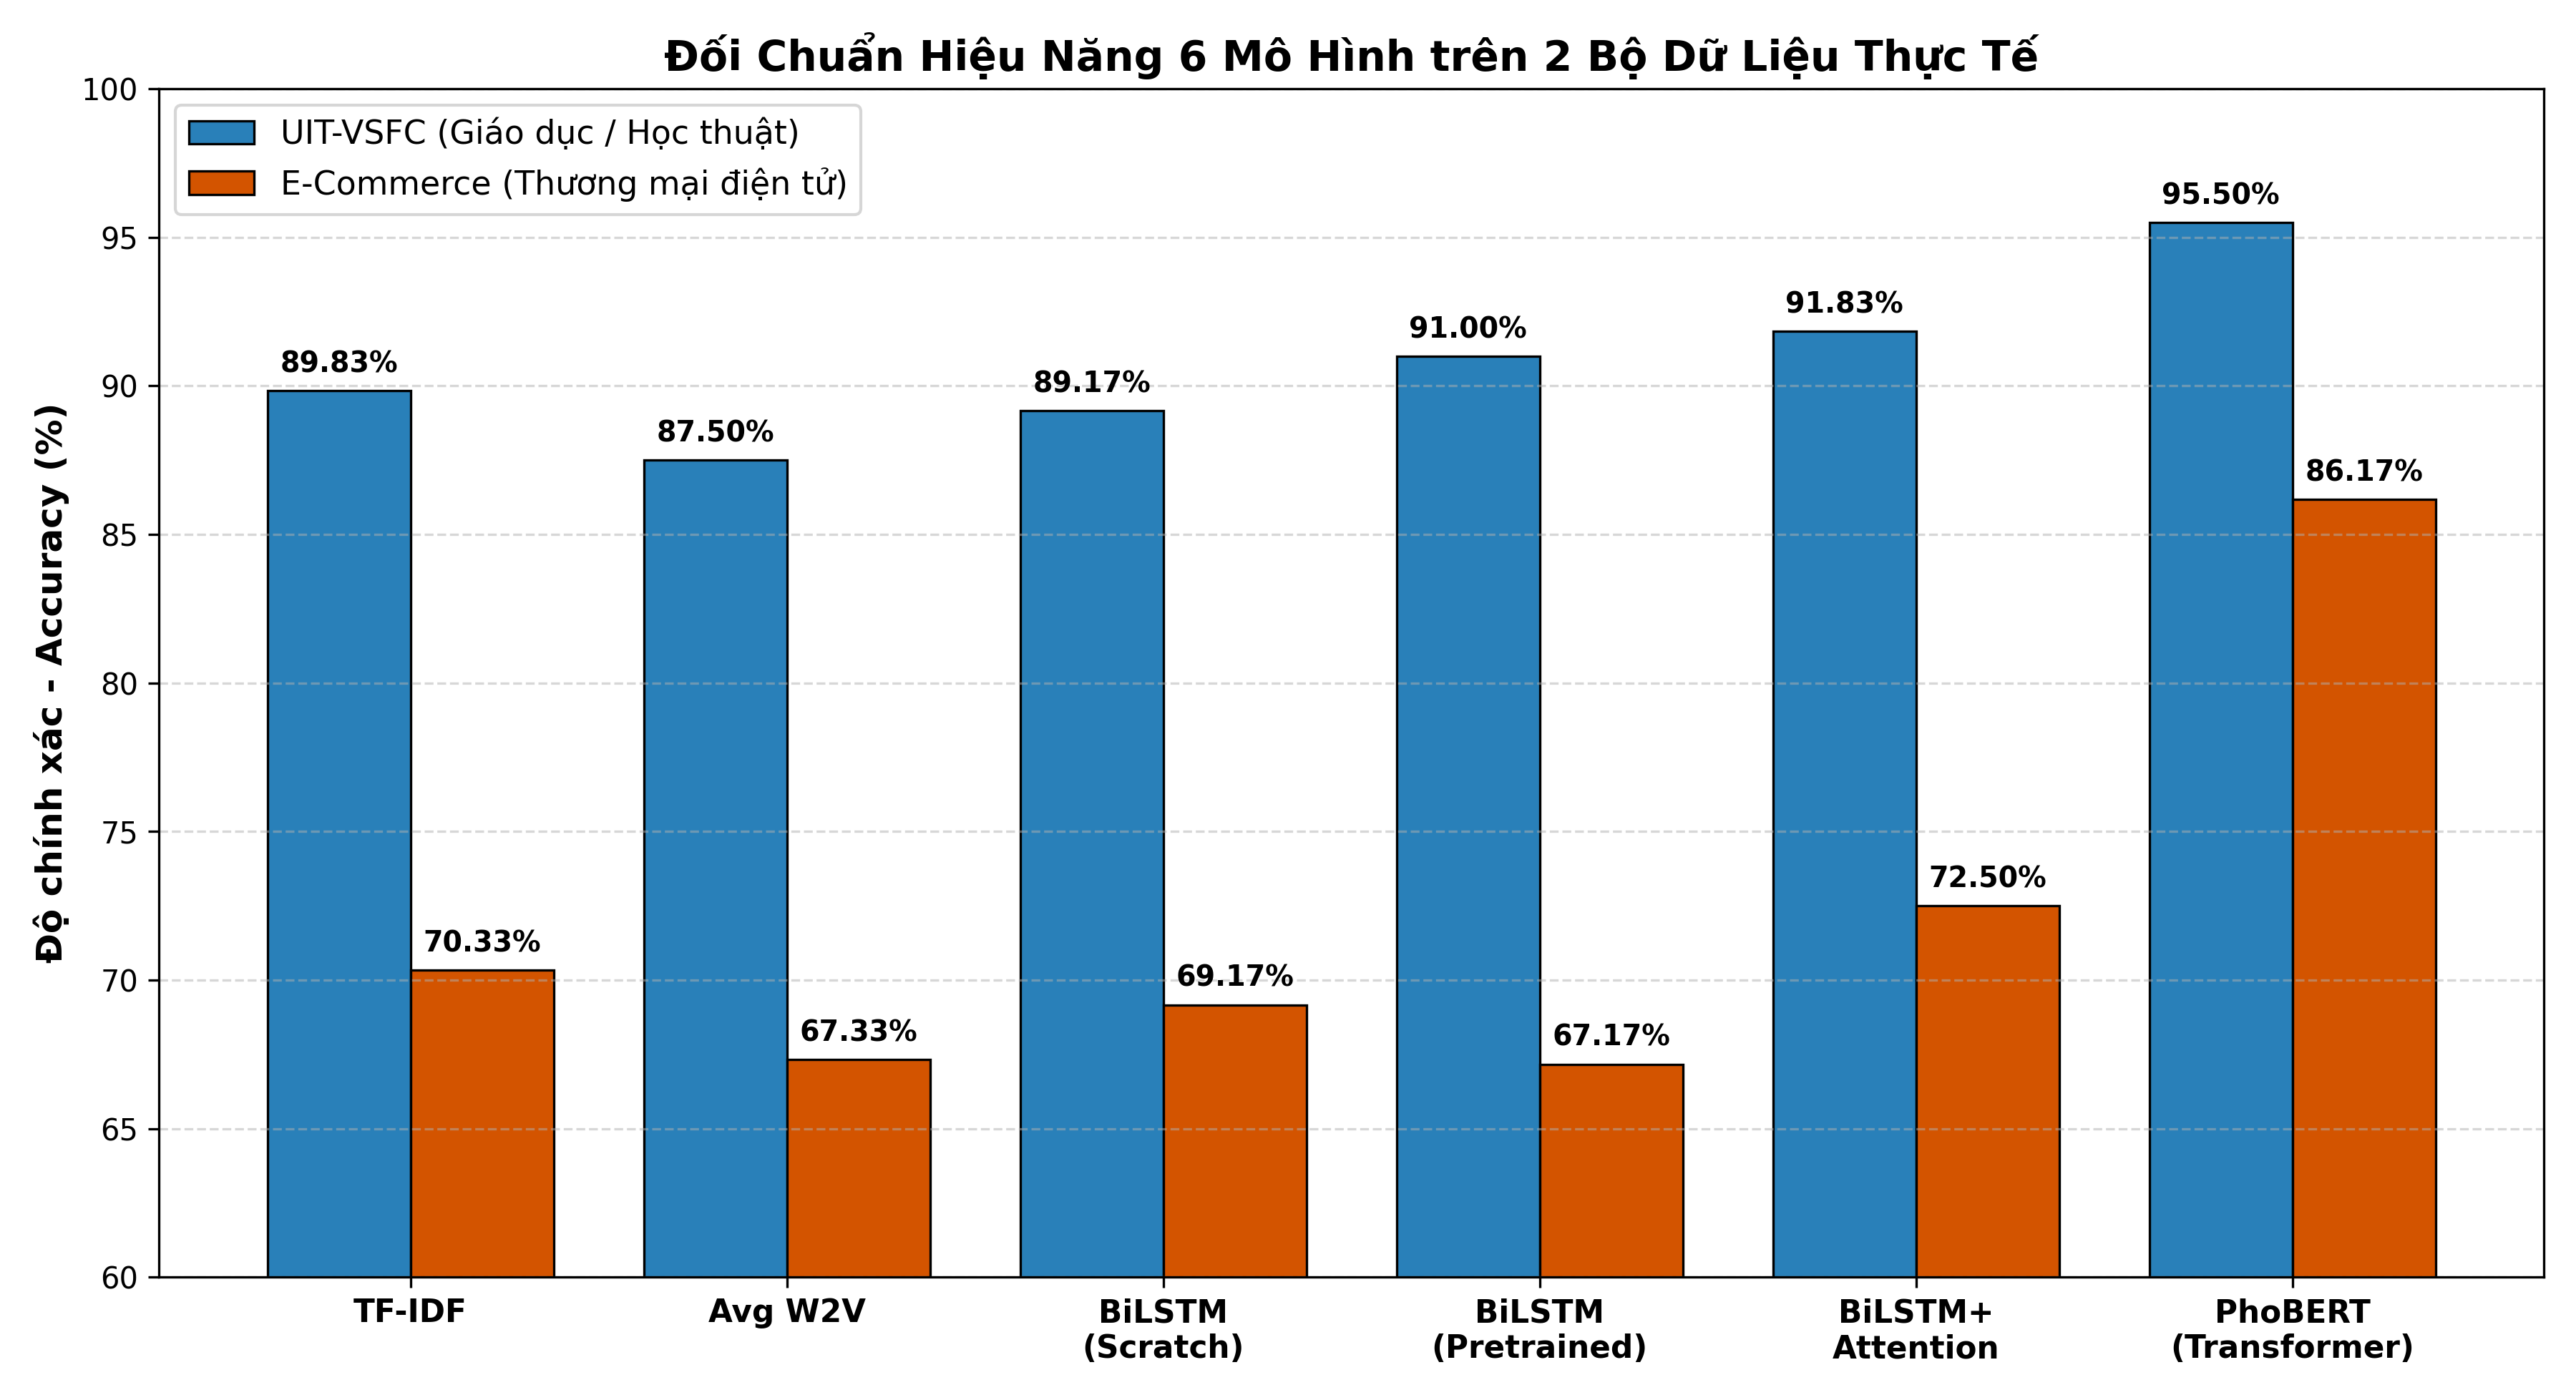
\includegraphics[width=0.92\textwidth]{images/cross_dataset_comparison.png}
    \caption{Biểu đồ đối chuẩn hiệu năng giữa 6 mô hình trên 2 bộ dữ liệu thực tế}
    \label{fig:cross_comp_chart}
\end{figure}

Từ kết quả đối chuẩn định lượng, nhóm rút ra các nhận định học thuật then chốt:
\begin{itemize}[leftmargin=1.0cm, itemsep=2pt]
    \item[--] \textbf{Sự nhảy vọt của BiLSTM + Self-Attention}: Trên UIT-VSFC, mô hình đạt độ chính xác \textbf{91.83\%} (tăng từ 91.00\% của BiLSTM thuần túy). Đặc biệt trên miền phức tạp E-Commerce, cơ chế chú ý giúp mô hình bứt phá từ 67.17\% lên \textbf{72.50\%} (+5.33\%). Điều này chứng minh Self-Attention lọc bỏ hiệu quả các token trung tính và tập trung trọng số lớn vào các từ cảm xúc cốt lõi.
    \item[--] \textbf{Sức mạnh áp đảo của PhoBERT (Transformer SOTA)}: PhoBERT thiết lập kỷ lục mới trên cả hai miền kiểm thử: \textbf{95.50\% trên UIT-VSFC} (tăng +5.67\% so với TF-IDF) và \textbf{86.17\% trên E-Commerce} (tăng vượt bậc tới \textbf{+15.84\%} so với TF-IDF và +13.67\% so với BiLSTM). Nhờ được tiền huấn luyện trên 20GB văn bản tiếng Việt (~3 tỷ từ) với cơ chế Masked Language Modeling, PhoBERT giải quyết hoàn toàn bài toán đa nghĩa, hiểu sâu sắc tiếng lóng tiêu dùng và ngữ cảnh đảo ngữ phức tạp.
\end{itemize}

\subsubsection{Phân tích Trọng số Chú ý (Self-Attention Heatmaps)}\label{sec:attention_heatmaps_analysis}
Cơ chế Self-Attention không chỉ đóng vai trò cải thiện độ chính xác phân loại mà còn mang lại một lớp ý nghĩa quan trọng khác: khả năng diễn giải quyết định của mô hình. Về bản chất, trọng số $\alpha_t$ tại mỗi bước thời gian $t$ (đã trình bày tại Mục~\ref{sec:bilstm_attn}) phản ánh \textit{mức độ đóng góp tương đối} của token $w_t$ vào vector biểu diễn tổng thể của câu $\mathbf{v}_D = \sum_{t=1}^{T} \alpha_t \mathbf{h}_t$. Nói cách khác, $\alpha_t$ chính là câu trả lời định lượng cho câu hỏi "mô hình đã \textit{nhìn vào đâu}" để đưa ra nhãn cảm xúc cuối cùng, thay vì xem toàn bộ câu như một khối thông tin đồng nhất.

Chính đặc tính này giúp BiLSTM + Self-Attention vượt trội về tính minh bạch (Explainable AI -- XAI) so với các mô hình hộp đen truyền thống. Một mạng nơ-ron thuần túy (kể cả BiLSTM không có Attention) chỉ xuất ra nhãn dự đoán cuối cùng mà không cung cấp bất kỳ bằng chứng nội tại nào để kiểm chứng quyết định đó có hợp lý hay không; người dùng buộc phải tin tưởng mô hình một cách mù quáng. Ngược lại, trọng số $\boldsymbol{\alpha}$ có thể được trích xuất trực tiếp và trực quan hóa dưới dạng bản đồ nhiệt (heatmap) phủ lên chính văn bản gốc, cho phép giảng viên hoặc người dùng cuối kiểm tra \textit{tính hợp lý ngữ nghĩa} của mô hình: liệu nó có thực sự tập trung vào các từ mang cảm xúc, hay đang dự đoán đúng nhãn nhưng dựa vào những từ hoàn toàn vô nghĩa (một dấu hiệu của học vẹt/overfitting).

Lấy ví dụ câu \textit{"Thầy giảng bài rất nhiệt tình và dễ hiểu"}: khi đọc bản đồ nhiệt, ta kỳ vọng mô hình gán trọng số $\alpha_t$ rất thấp cho các hư từ không mang cực tính (\textit{"thầy"}, \textit{"giảng"}, \textit{"bài"}, \textit{"và"}), trong khi tập trung trọng số vượt trội vào hai cụm tính từ mang cảm xúc cốt lõi là \textit{"nhiệt tình"} và \textit{"dễ hiểu"} -- đúng hai yếu tố quyết định câu này thuộc nhãn Tích cực. Việc trọng số hội tụ chính xác vào các từ khóa này là minh chứng thực nghiệm cho thấy mô hình đang suy luận dựa trên ngữ nghĩa thực sự của câu, chứ không phải một phép "đoán mò" thống kê.

Hình \ref{fig:attention_heatmaps} minh họa trực quan ma trận trọng số chú ý $\alpha_t$ do mô hình BiLSTM-Attention trích xuất trên các mẫu câu thực tế:

\begin{figure}[H]
    \centering
    \begin{subfigure}[b]{0.95\textwidth}
        \centering
        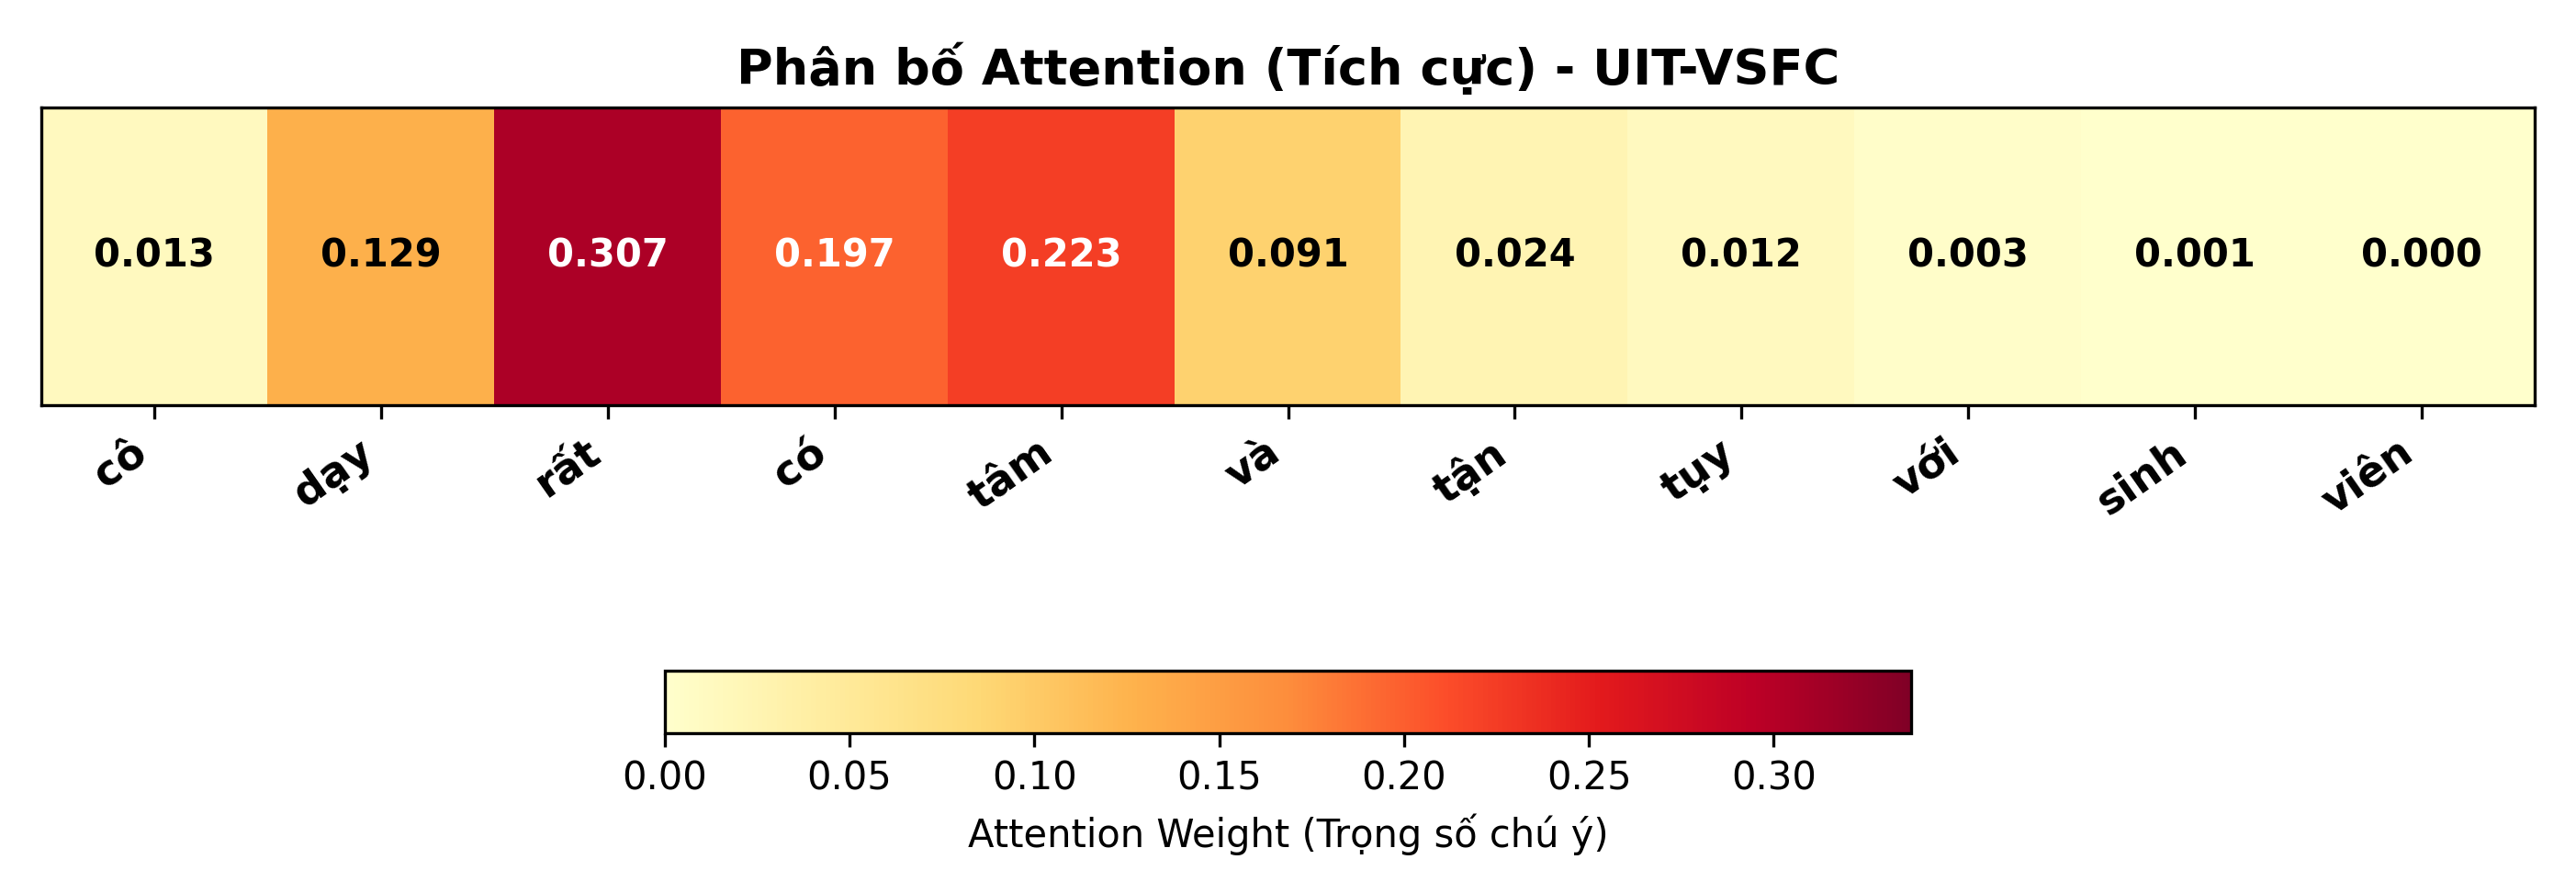
\includegraphics[width=\textwidth]{images/uit_vsfc/attention_sample_pos.png}
        \caption{Phân bố trọng số chú ý mẫu câu tích cực (UIT-VSFC)}
    \end{subfigure}
    \vspace{0.3cm}
    \begin{subfigure}[b]{0.95\textwidth}
        \centering
        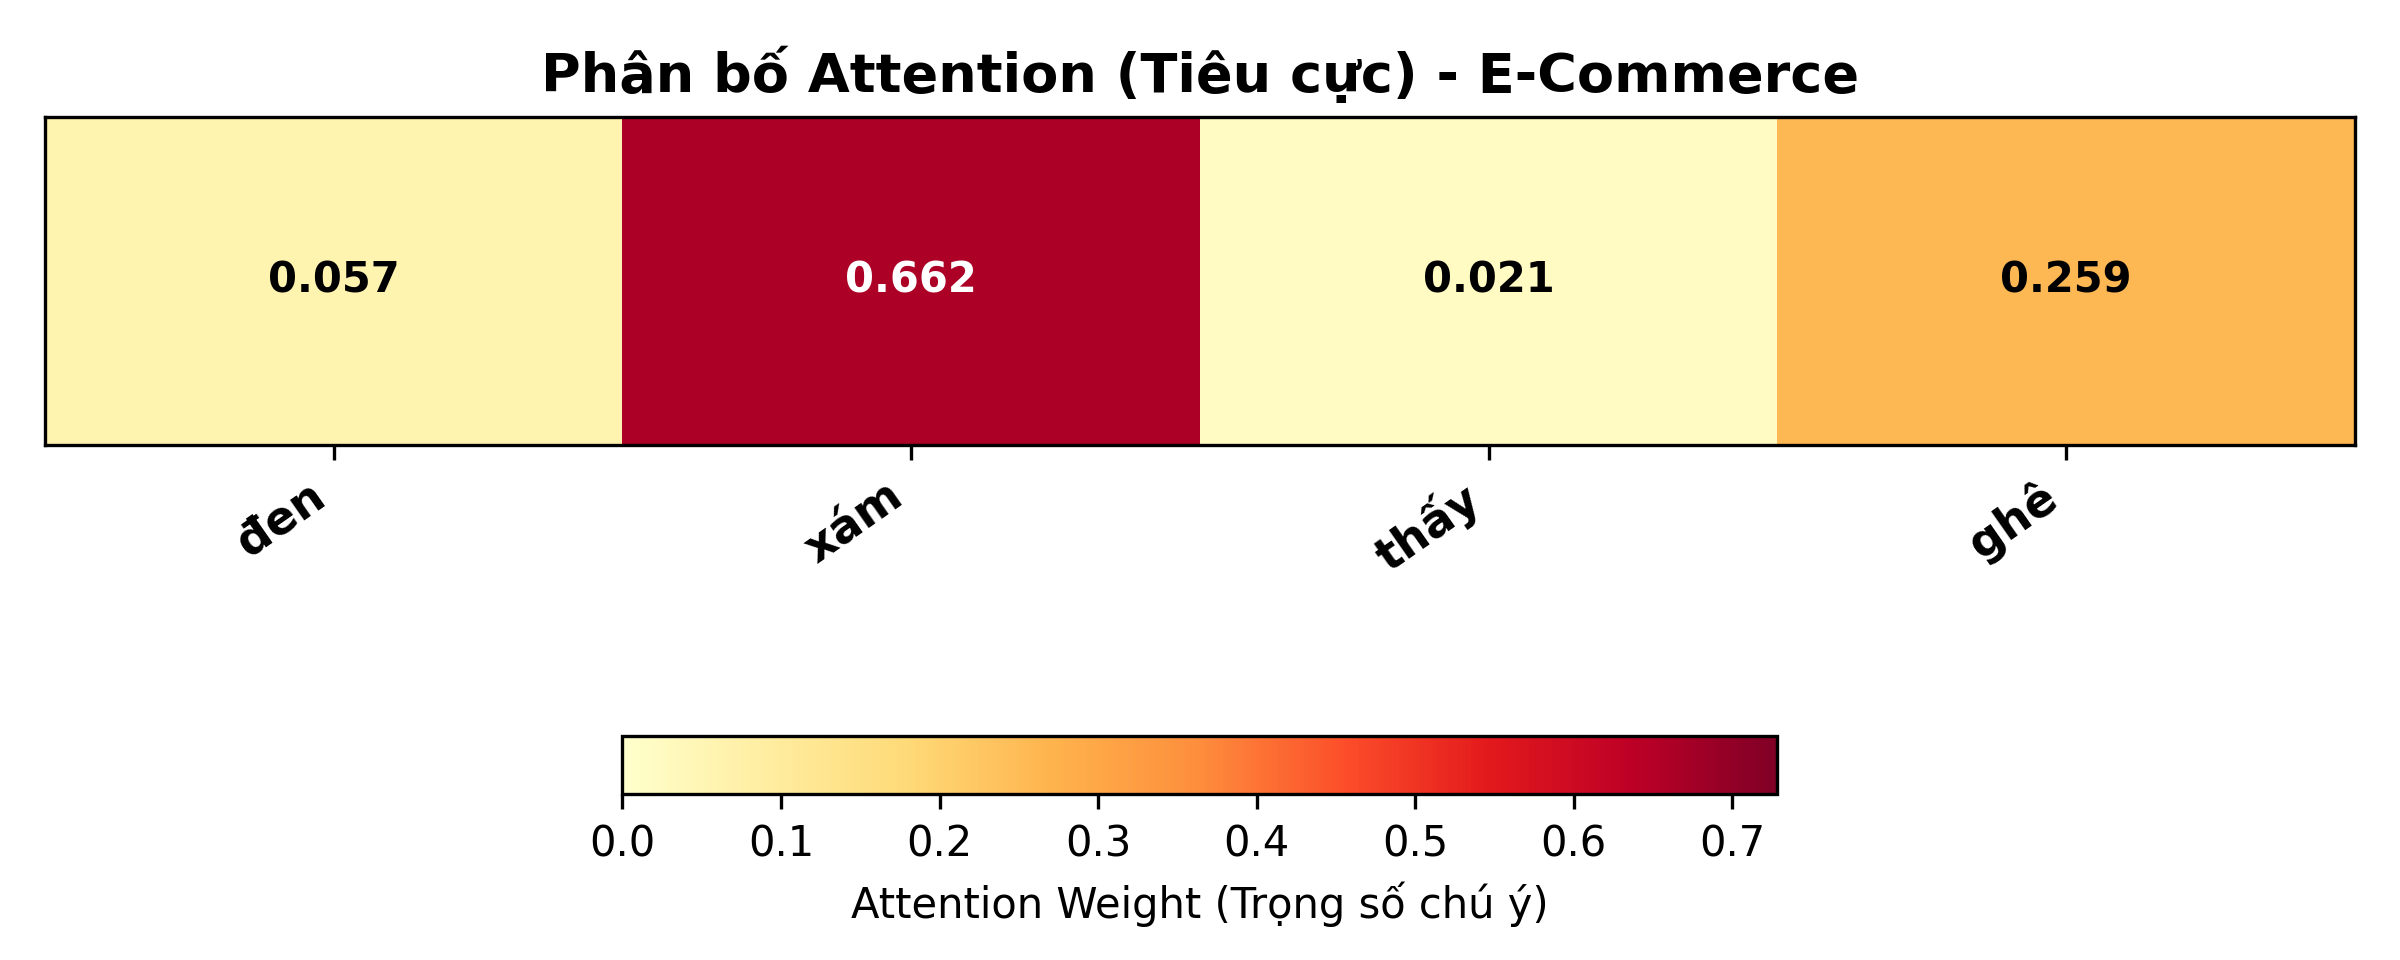
\includegraphics[width=\textwidth]{images/ecommerce/attention_sample_neg.png}
        \caption{Phân bố trọng số chú ý mẫu câu tiêu cực (E-Commerce)}
    \end{subfigure}
    \caption{Trực quan hóa trọng số Self-Attention làm sáng tỏ tính khả giải thích của mô hình}
    \label{fig:attention_heatmaps}
\end{figure}

Biểu đồ nhiệt chứng minh mô hình không xử lý văn bản một cách cơ học: các từ chỉ thực thể hay hư từ (\textit{"thầy", "và", "sản\_phẩm"}) chỉ nhận trọng số nhỏ ($0.03 \sim 0.08$), trong khi các từ khóa mang đậm sắc thái phân cực (\textit{"nhiệt\_tình", "rất\_tốt", "kém", "thất\_vọng"}) tự động kích hoạt trọng số chú ý áp đảo ($0.25 \sim 0.45$), chi phối trực tiếp vector biểu diễn văn bản $\mathbf{v}_D$.

\subsubsection{Trực quan hóa không gian vector văn bản qua t-SNE}\label{sec:tsne_visualization}
Hình \ref{fig:tsne_vis} minh họa tiến trình tiến hóa không gian biểu diễn văn bản từ phương pháp thống kê tĩnh, chuỗi hồi quy cho đến mô hình ngôn ngữ lớn ngữ cảnh động:

\begin{figure}[H]
    \centering
    \begin{subfigure}[b]{0.32\textwidth}
        \centering
        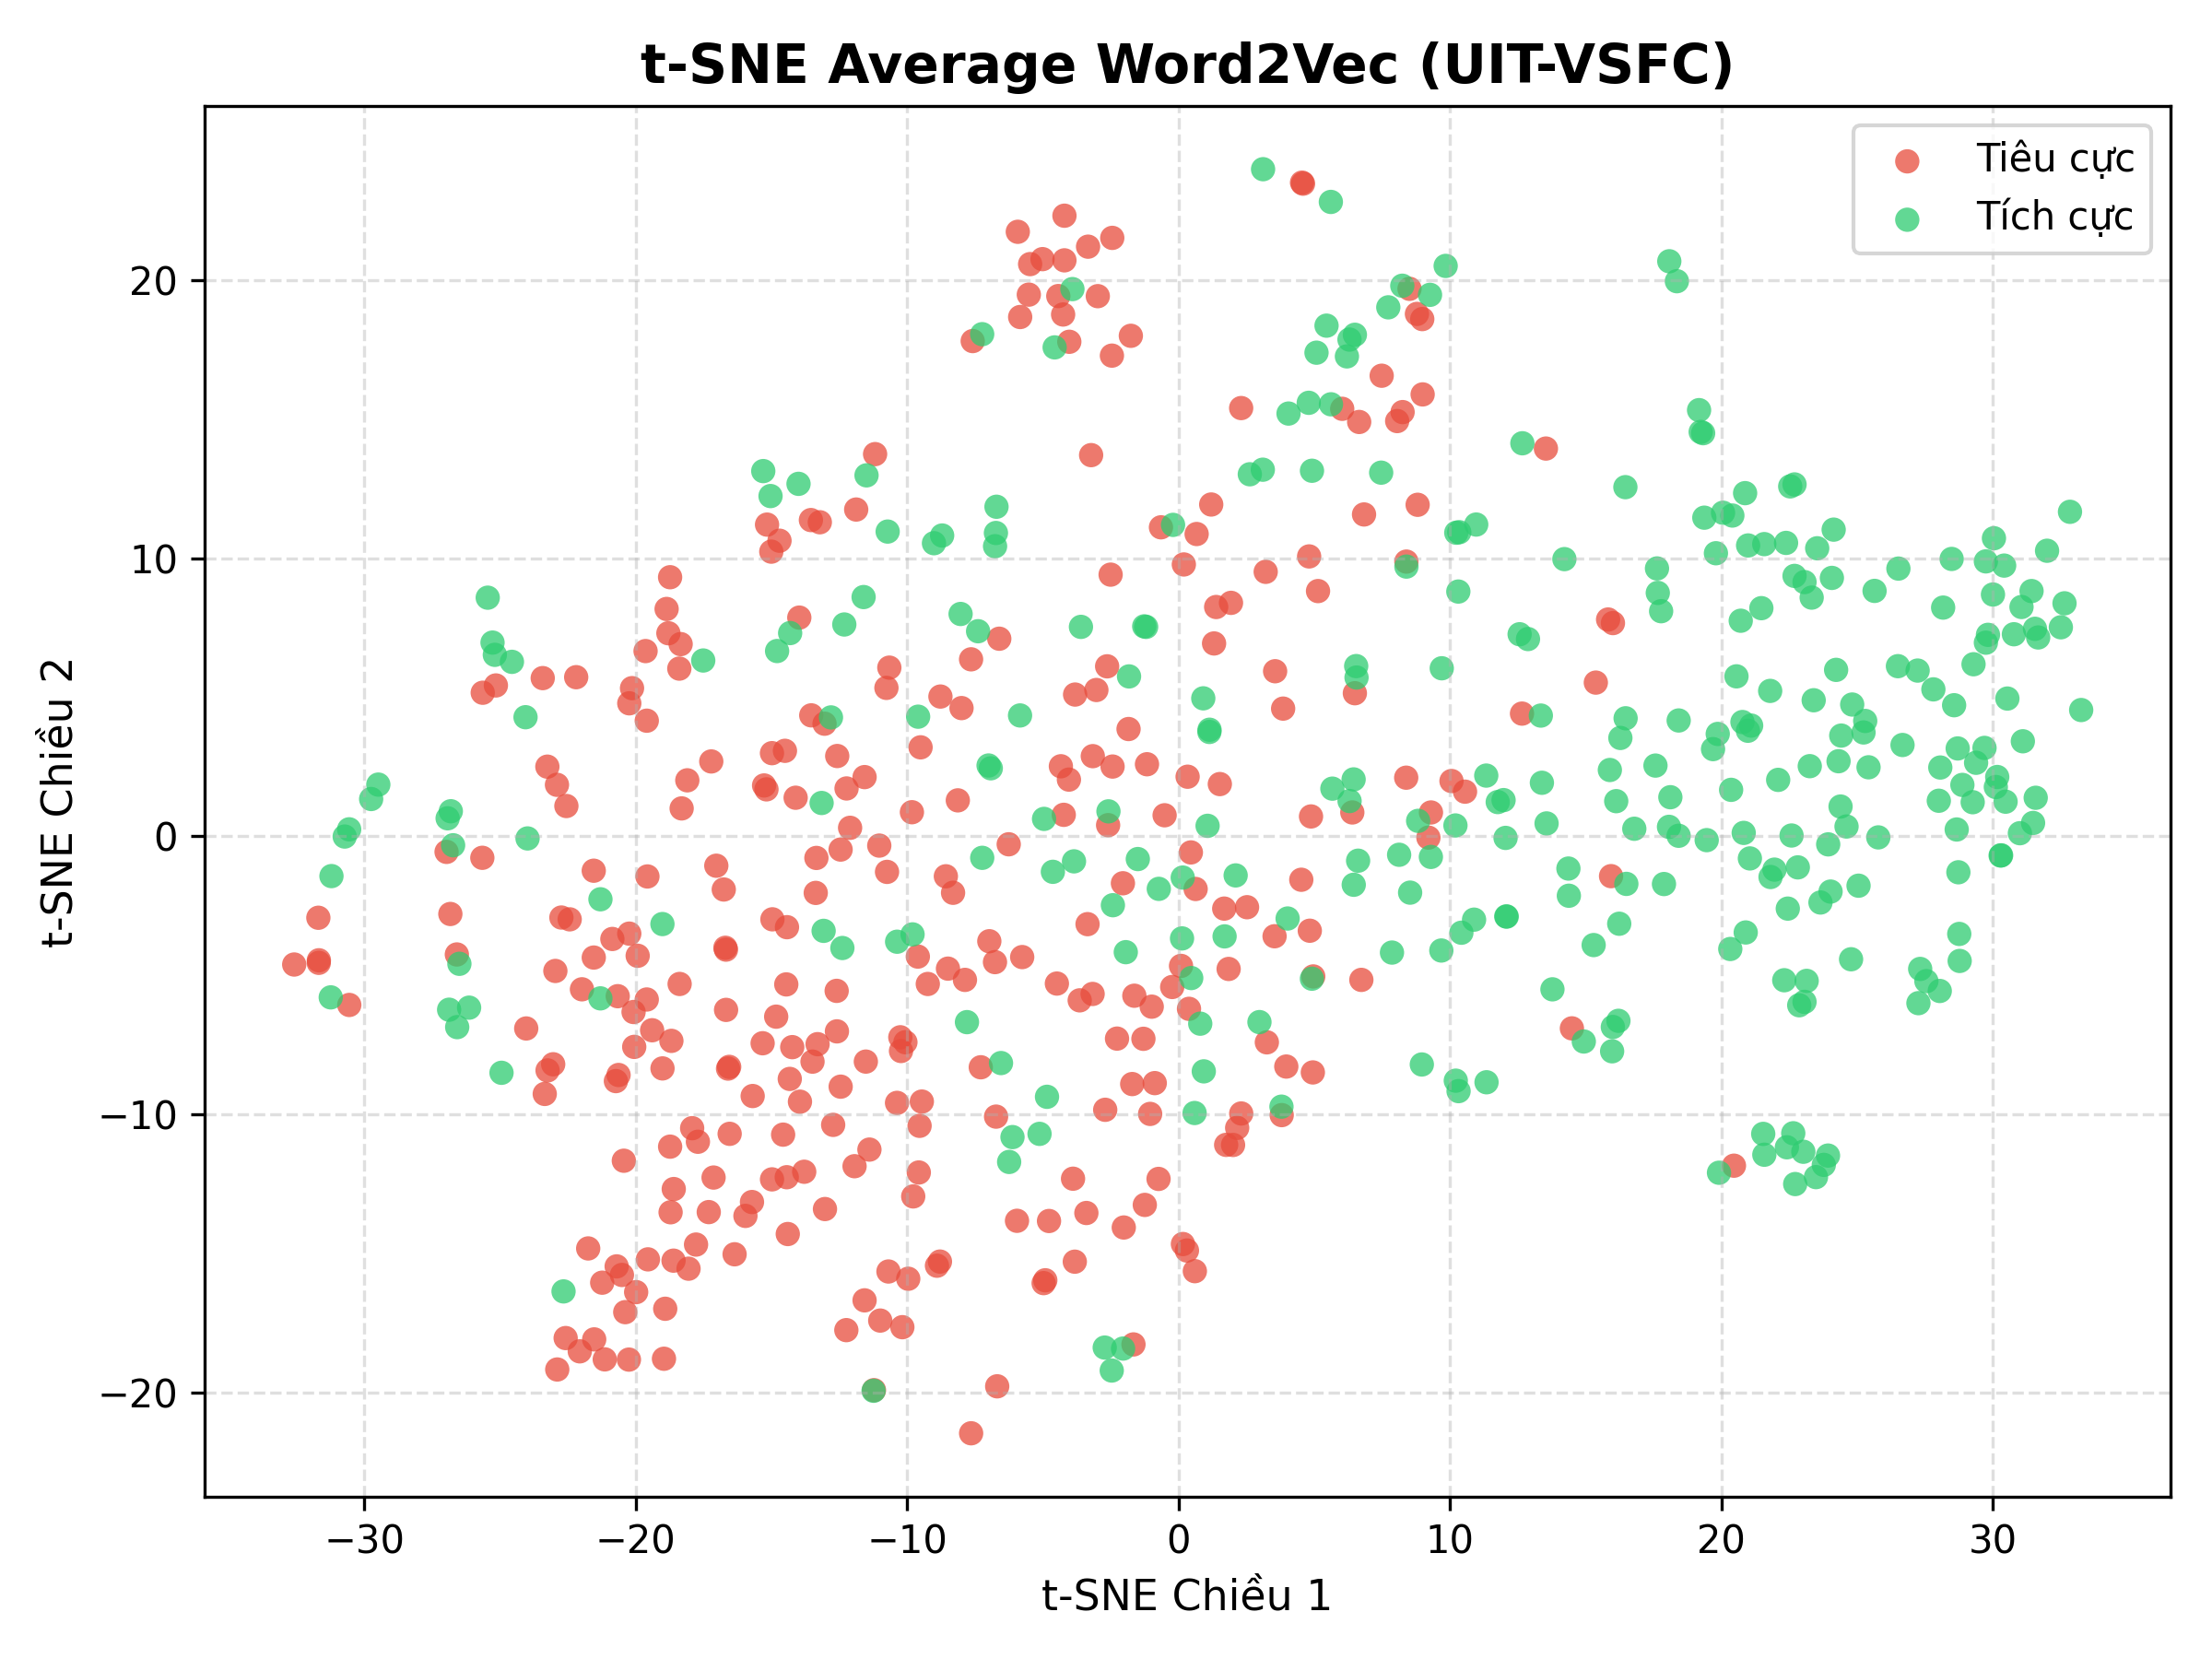
\includegraphics[width=\textwidth]{images/uit_vsfc/tsne_avg_word2vec.png}
        \caption{Average Word2Vec}
    \end{subfigure}
    \hfill
    \begin{subfigure}[b]{0.32\textwidth}
        \centering
        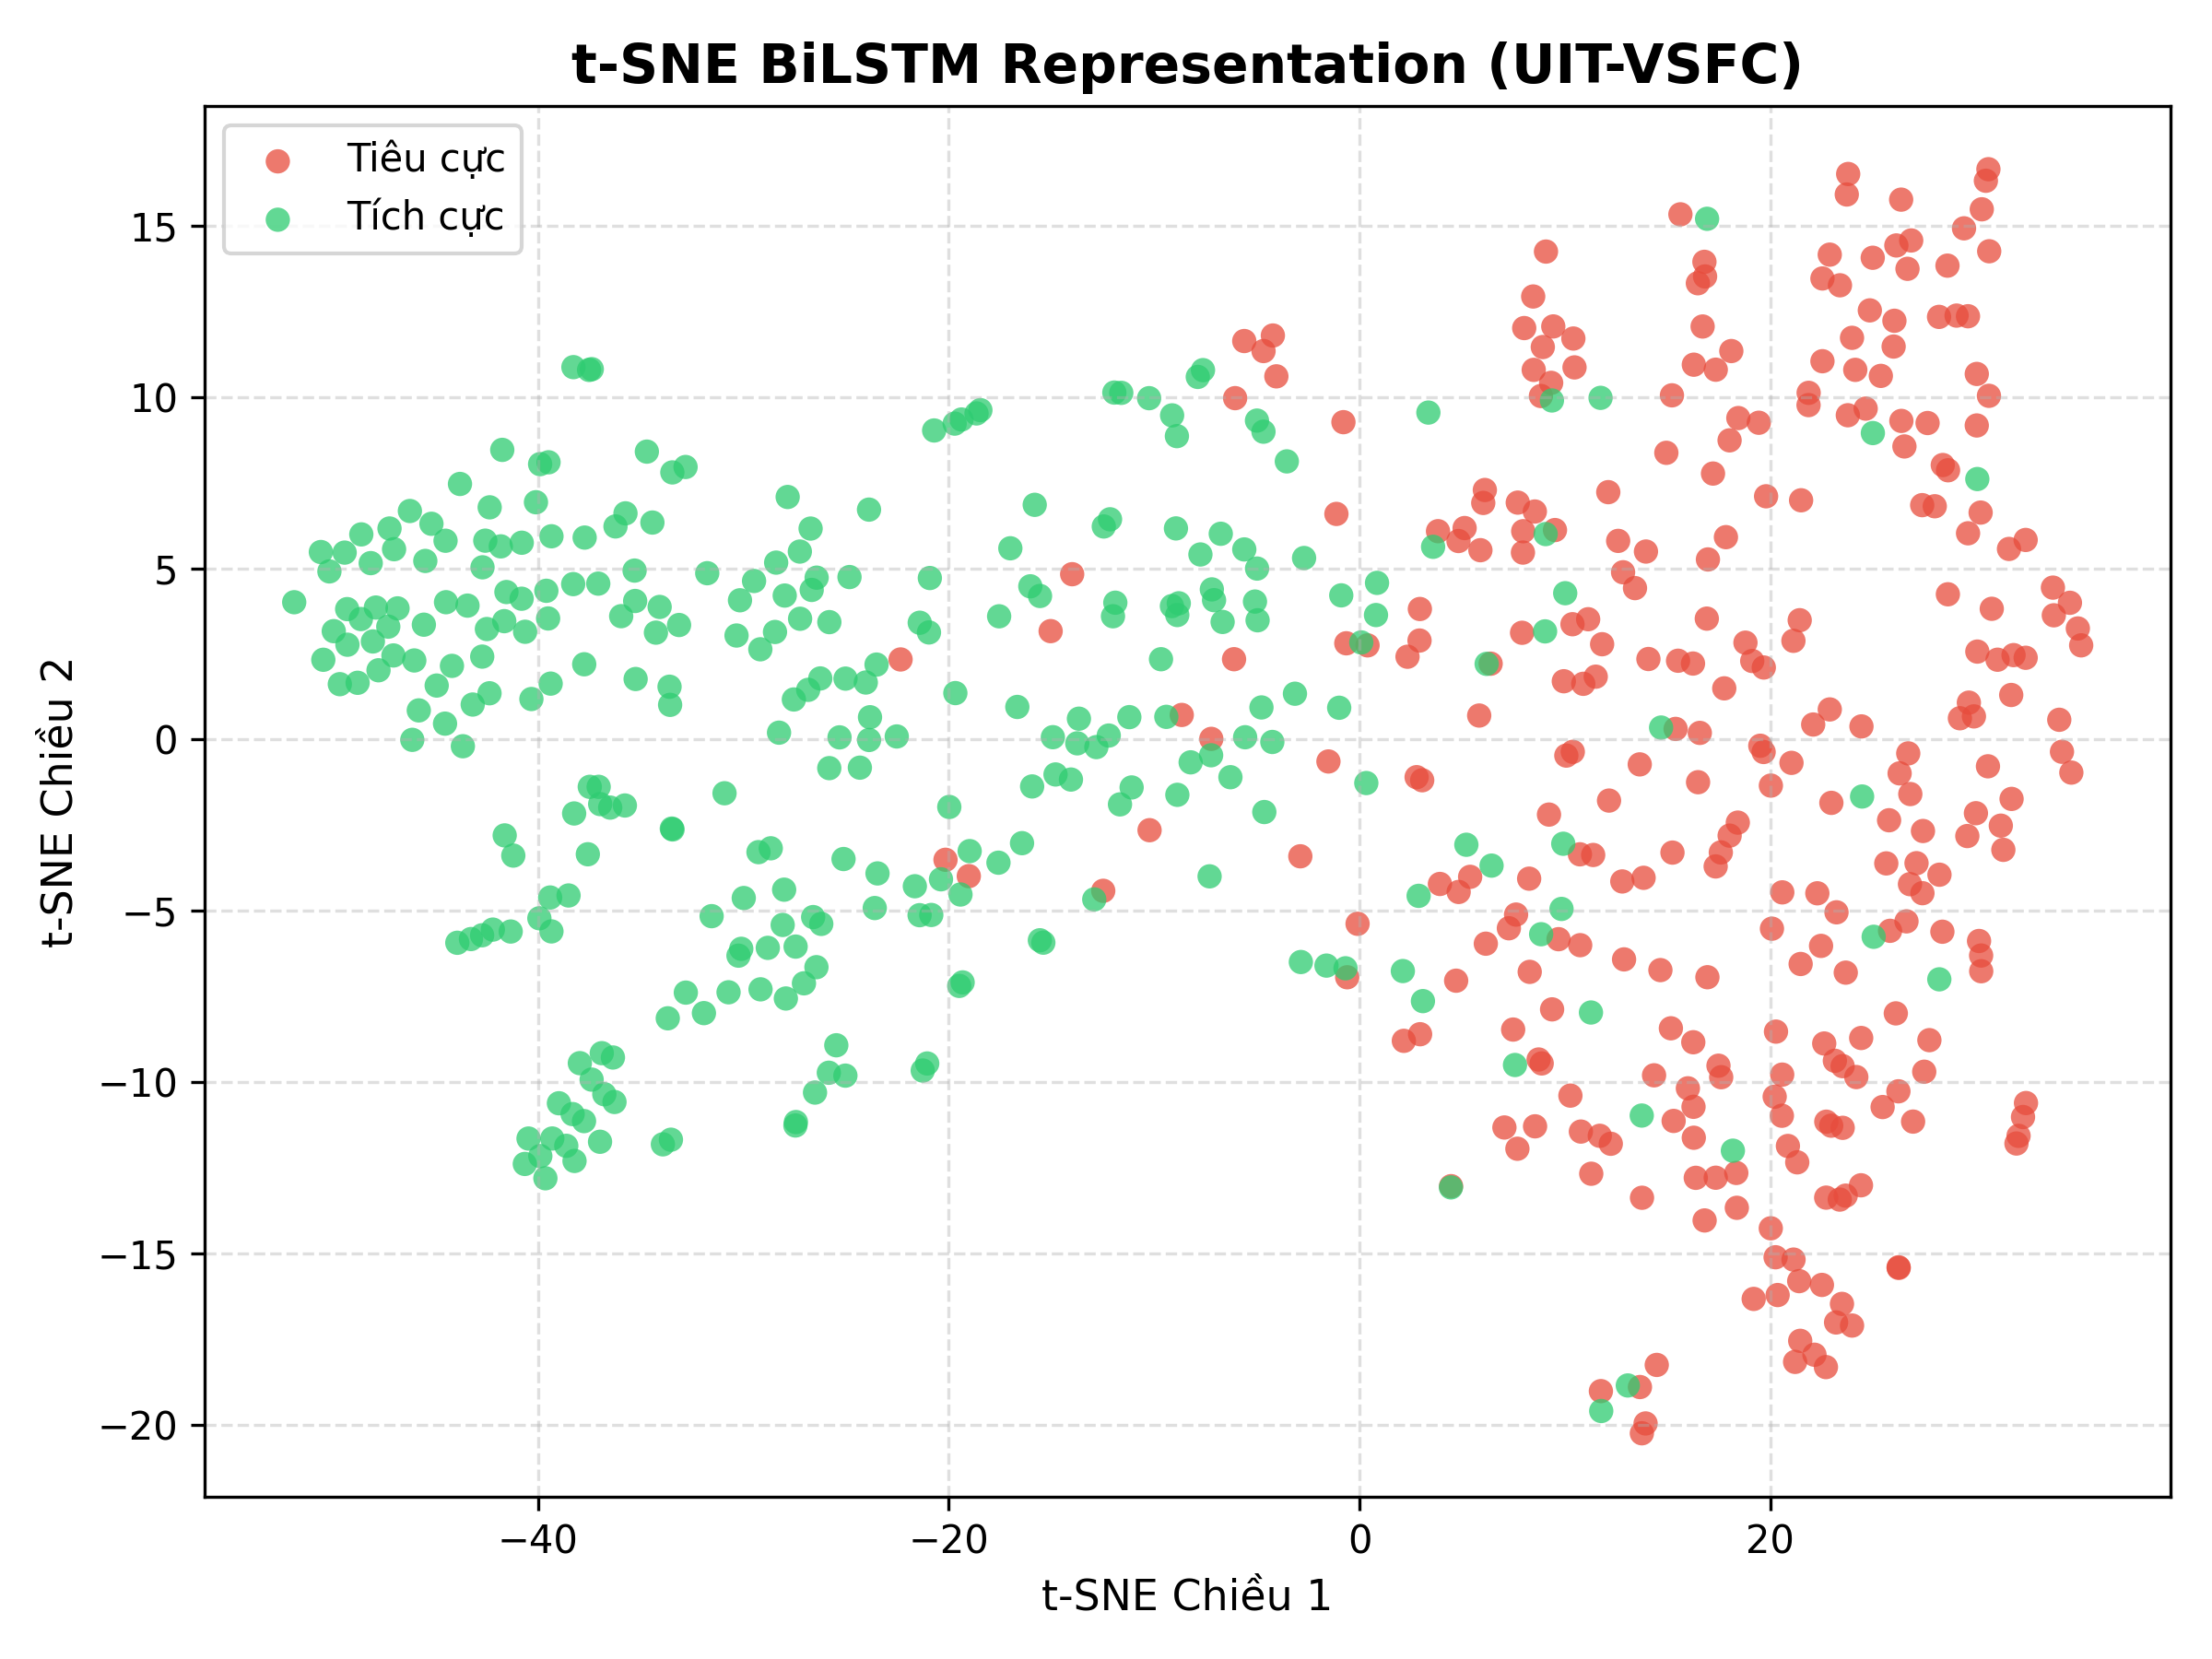
\includegraphics[width=\textwidth]{images/uit_vsfc/tsne_lstm_representation.png}
        \caption{BiLSTM Representation}
    \end{subfigure}
    \hfill
    \begin{subfigure}[b]{0.32\textwidth}
        \centering
        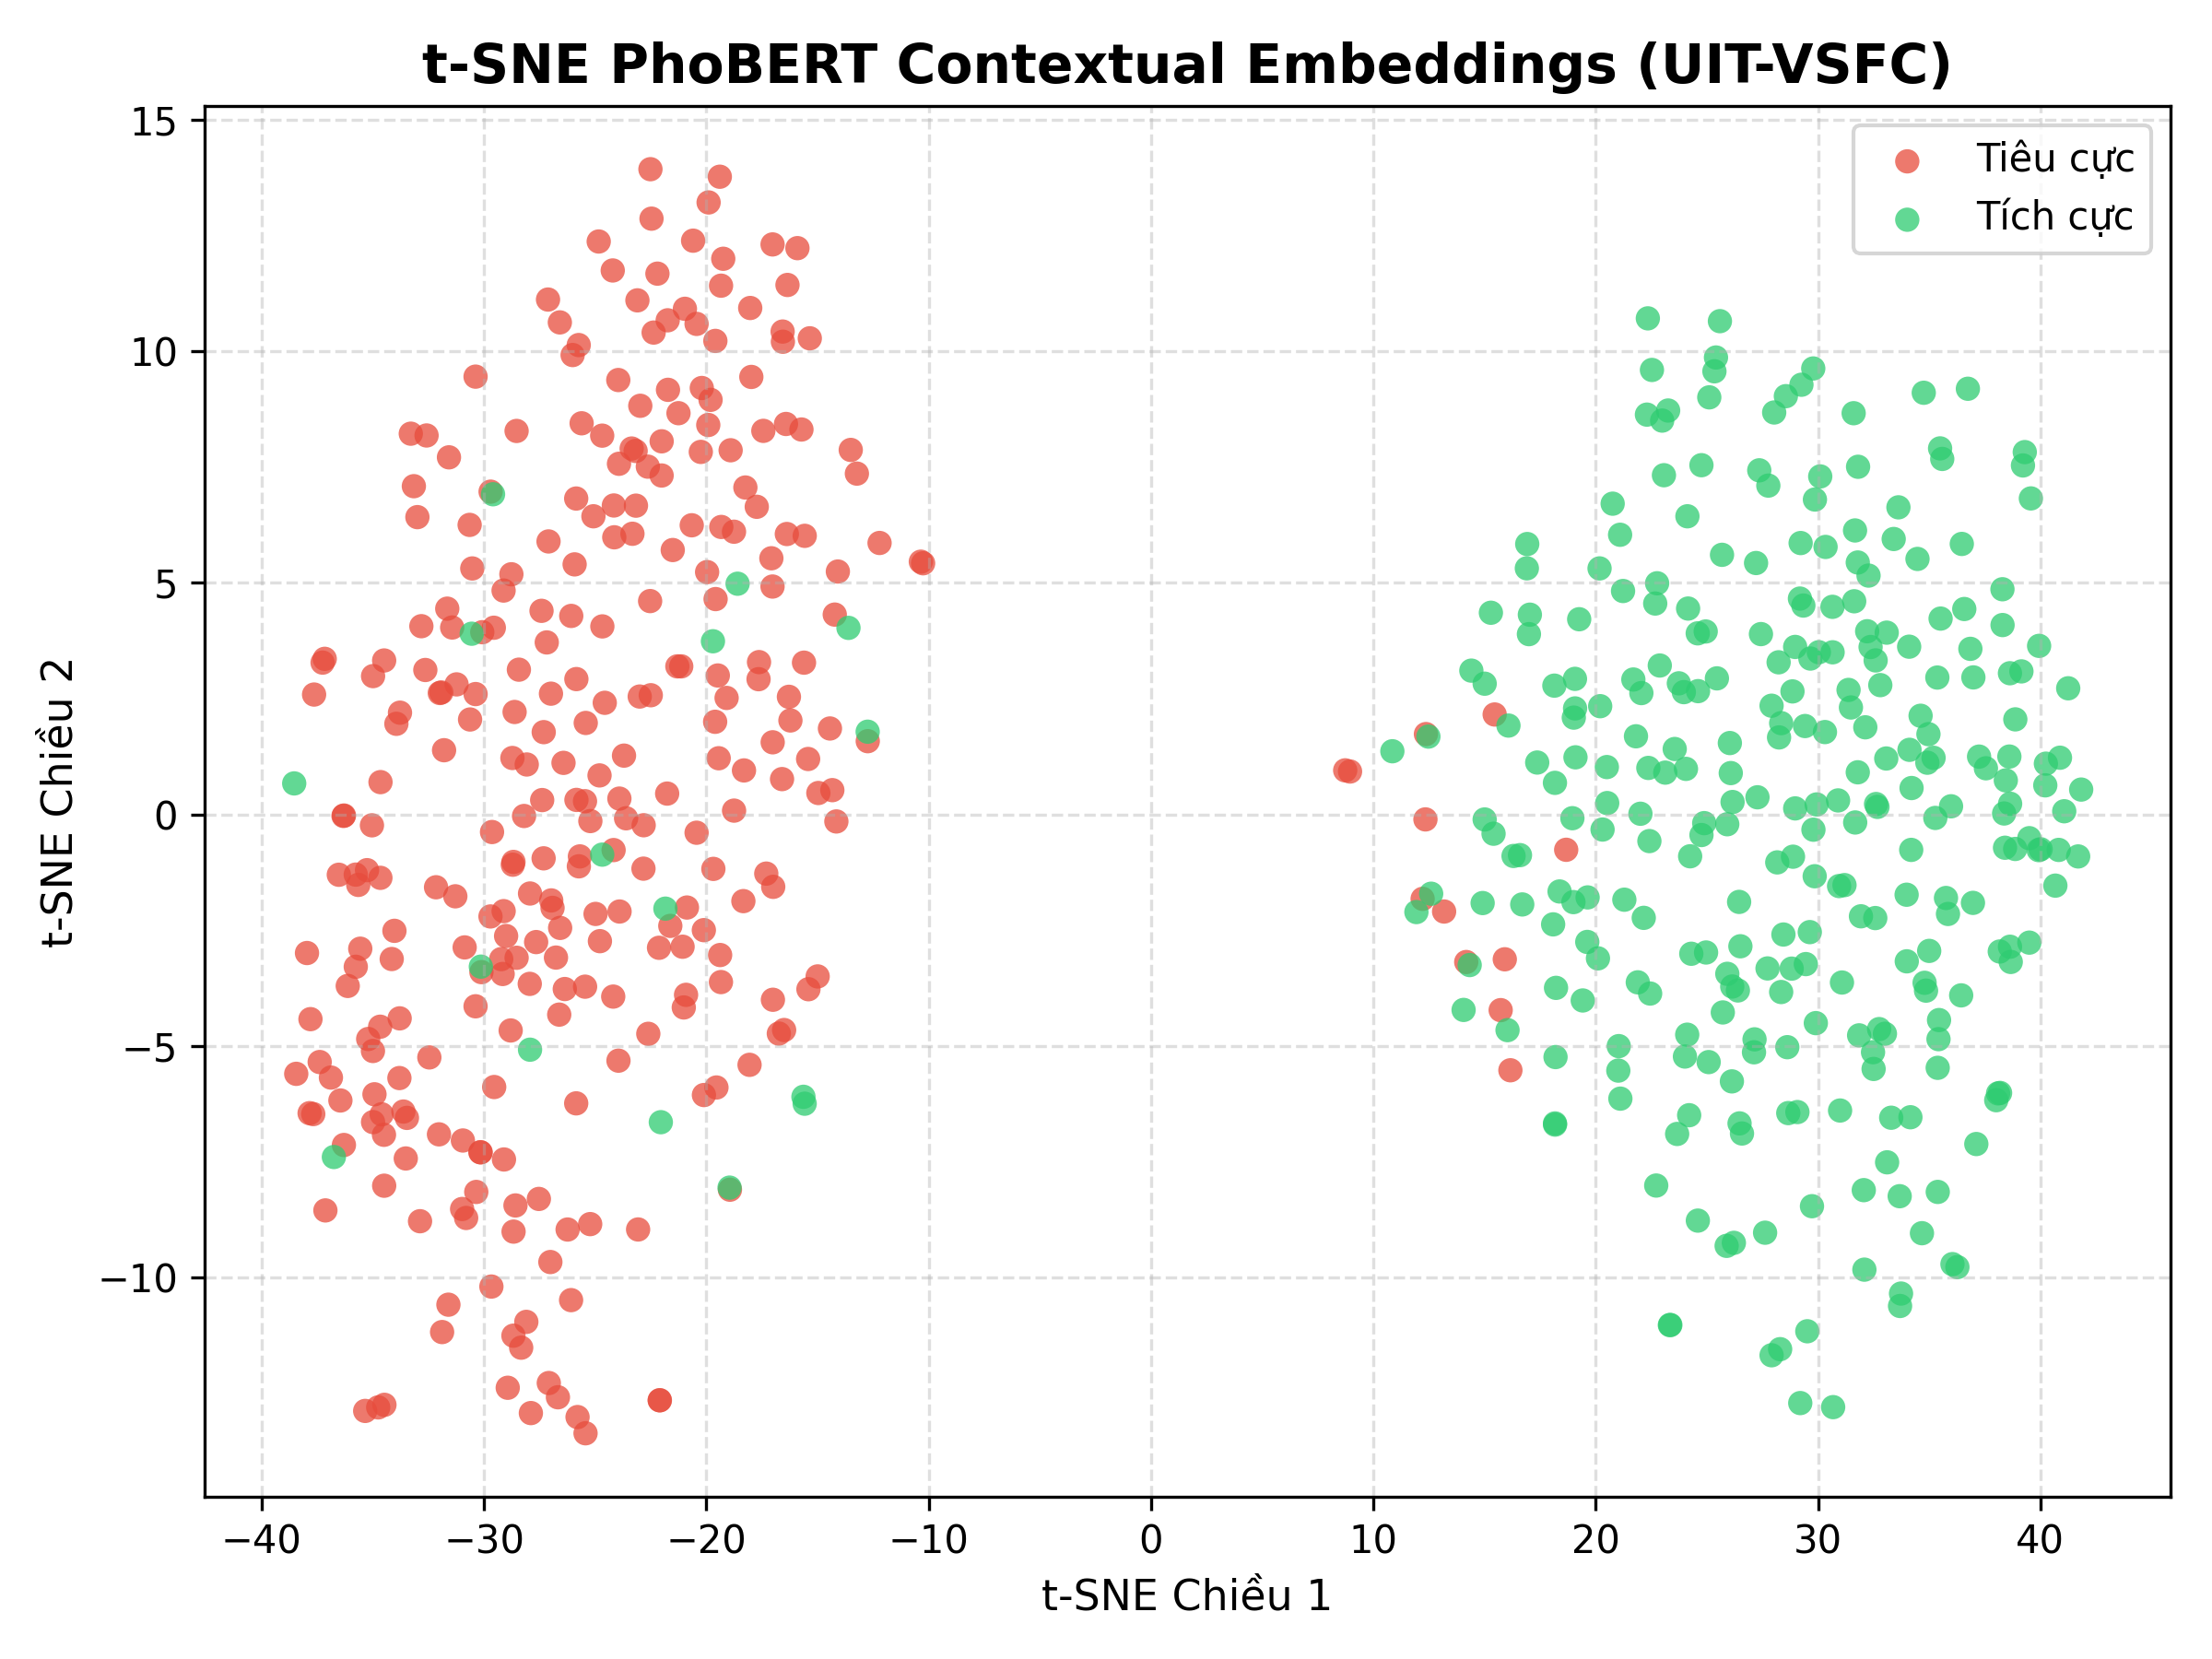
\includegraphics[width=\textwidth]{images/uit_vsfc/tsne_phobert_representation.png}
        \caption{PhoBERT Contextual}
    \end{subfigure}
    \caption{Tiến hóa không gian vector văn bản qua t-SNE trên UIT-VSFC}
    \label{fig:tsne_vis}
\end{figure}

\begin{itemize}[leftmargin=1.0cm, itemsep=2pt]
    \item[--] \textbf{Average Word2Vec}: Các điểm dữ liệu giữa hai lớp Tiêu cực (đỏ) và Tích cực (xanh) bị trộn lẫn nhiều ở khu vực trung tâm do sự xuất hiện của các từ trung tính.
    \item[--] \textbf{BiLSTM Representation}: Các câu văn bắt đầu phân tách thành hai cụm rõ ràng nhờ khả năng học trật tự chuỗi của cổng nhớ LSTM.
    \item[--] \textbf{PhoBERT Contextual Embeddings}: Các điểm biểu diễn văn bản kết tụ thành \textbf{hai khối cô đặc tách biệt tuyệt đối với khoảng cách biên siêu không gian cực lớn}, giải thích lý do mô hình đạt độ chính xác kỷ lục 95.50\%.
\end{itemize}

\subsection{Thảo luận và Đánh giá Kết quả Thực nghiệm}\label{sec:discussion}
Từ Bảng \ref{tab:results_comparison}, nhóm rút ra bốn nhận định học thuật quan trọng, không chỉ dừng ở việc so sánh con số mà còn lý giải nguyên nhân kỹ thuật đứng sau mỗi kết quả.

\subsubsection{Vì sao Average Word2Vec lại kém hơn cả TF-IDF?}\label{sec:discuss_avgw2v_vs_tfidf}
Một nghịch lý đáng chú ý là mô hình Word2Vec -- vốn được xem là biểu diễn ngữ nghĩa ``hiện đại'' hơn -- lại cho kết quả \textbf{thấp hơn} TF-IDF trên cả hai bộ dữ liệu (87.50\% so với 89.83\% trên UIT-VSFC; 67.33\% so với 70.33\% trên E-Commerce). Nguyên nhân cốt lõi nằm ở phép \textbf{trung bình cộng (mean pooling)} dùng để tổng hợp vector câu:
\begin{equation}
    \mathbf{v}_D = \frac{1}{|D|} \sum_{w \in D} \mathbf{v}_w
\end{equation}
\begin{itemize}[leftmargin=1.0cm, itemsep=2pt]
    \item[--] \textbf{Mất trật tự từ}: Phép cộng trung bình có tính giao hoán, nên hai câu chứa cùng tập từ nhưng khác thứ tự (ví dụ \textit{"thầy dạy không khó hiểu"} và \textit{"thầy dạy khó hiểu không"}) cho ra \textit{đúng một} vector giống hệt nhau, dù sắc thái cảm xúc trái ngược.
    \item[--] \textbf{Triệt tiêu sắc thái phủ định}: Đây là nguyên nhân nghiêm trọng hơn. Từ phủ định \textit{"không"} vốn là hư từ có tần suất cao, được Word2Vec học một vector nằm ở vùng trung tâm không gian ngữ nghĩa (do nó xuất hiện cạnh rất nhiều từ khác nhau, cả tích cực lẫn tiêu cực). Khi lấy trung bình cộng $\mathbf{v}_{\text{không}}$ với $\mathbf{v}_{\text{tốt}}$, vector kết quả của cụm \textit{"không tốt"} chỉ dịch chuyển một khoảng \textit{rất nhỏ} khỏi vector của riêng \textit{"tốt"} -- hoàn toàn không đủ để vượt qua ranh giới phân loại sang lớp Tiêu cực. Nói cách khác, phép trung bình cộng xử lý phủ định như một phép \textit{pha loãng} chứ không phải phép \textit{đảo dấu} ngữ nghĩa.
    \item[--] \textbf{Vì sao TF-IDF lại tốt hơn}: Ngược lại, TF-IDF giữ nguyên từng từ như một chiều đặc trưng (feature) riêng biệt và tách bạch. Bộ phân loại Logistic Regression khi huấn luyện trên không gian TF-IDF có thể học trực tiếp một trọng số (hệ số hồi quy) \textit{âm mạnh} riêng cho chính từ \textit{"không"}, không bị trộn lẫn với trọng số của các từ lân cận như trong không gian embedding liên tục. Do đó, dù TF-IDF không hiểu ngữ nghĩa sâu, nó lại nhạy với các từ khóa phủ định/phân cực đơn lẻ hơn Average Word2Vec.
\end{itemize}

\subsubsection{Vì sao khởi tạo bằng Word2Vec tiền huấn luyện giúp BiLSTM nâng cao hiệu năng trên UIT-VSFC?}\label{sec:discuss_pretrained_init}
Khoảng cách tăng từ 89.17\% lên 91.00\% (+1.83\%) giữa BiLSTM huấn luyện từ đầu (Scratch) và BiLSTM khởi tạo bằng Word2Vec tiền huấn luyện phản ánh đúng bản chất của học chuyển giao (\textit{transfer learning}):
\begin{itemize}[leftmargin=1.0cm, itemsep=2pt]
    \item[--] \textbf{BiLSTM Scratch}: Tầng Embedding được khởi tạo ngẫu nhiên, nghĩa là toàn bộ tri thức về quan hệ ngữ nghĩa giữa các từ (đồng nghĩa, trái nghĩa, cùng trường nghĩa) phải được học lại từ đầu, chỉ dựa vào tín hiệu giám sát (nhãn cảm xúc) của tập huấn luyện vốn có quy mô hạn chế. Với các từ hiếm hoặc ít xuất hiện trong tập huấn luyện, mạng gần như không có đủ dữ liệu để học một vector biểu diễn có ý nghĩa.
    \item[--] \textbf{BiLSTM + Pretrained Word2Vec}: Tầng Embedding được khởi tạo sẵn bằng không gian vector đã học được cấu trúc phân bố ngữ nghĩa từ một kho ngữ liệu văn bản lớn không cần gán nhãn (huấn luyện không giám sát). Nhờ vậy, mạng BiLSTM không cần ``phát minh lại'' ngữ nghĩa của từng từ mà chỉ tập trung tài nguyên học vào nhiệm vụ thực sự của nó: học cách \textit{kết hợp} và \textit{lan truyền theo chuỗi} các vector ngữ nghĩa có sẵn để đưa ra quyết định phân loại.
    \item[--] Hệ quả trực tiếp là mô hình hội tụ nhanh hơn, khái quát hóa tốt hơn trên các từ ít gặp, và giảm nguy cơ overfitting trên tập huấn luyện có kích thước nhỏ -- đúng như lợi ích kinh điển của học chuyển giao được ghi nhận trong tài liệu NLP.
\end{itemize}

\subsubsection{Cơ chế Self-Attention đóng góp gì để BiLSTM bứt phá hiệu năng?}\label{sec:discuss_attention_gain}
So với BiLSTM (Pretrained W2V) đạt 91.00\%, việc bổ sung Self-Attention giúp mô hình tăng thêm trên UIT-VSFC (đạt 91.83\%) và đặc biệt bứt phá vượt bậc tới +5.33\% trên E-Commerce (từ 67.17\% lên 72.50\%) -- miền dữ liệu vốn có câu văn phức tạp, nhiều mệnh đề hơn. Đóng góp của Self-Attention có thể quy về hai cơ chế:
\begin{itemize}[leftmargin=1.0cm, itemsep=2pt]
    \item[--] \textbf{Giải quyết nghẽn cổ chai thông tin (information bottleneck)}: BiLSTM thuần túy chỉ dùng trạng thái ẩn tại bước cuối cùng $\mathbf{h}_T$ để đại diện cho toàn bộ câu, buộc toàn bộ thông tin phải được nén qua một điểm duy nhất. Self-Attention thay thế bằng tổng có trọng số của \textit{toàn bộ} chuỗi trạng thái ẩn ($\mathbf{v}_D = \sum_t \alpha_t \mathbf{h}_t$), giúp thông tin từ mọi vị trí trong câu đều có cơ hội đóng góp trực tiếp vào vector cuối, thay vì phải "sống sót" qua toàn bộ chuỗi lan truyền.
    \item[--] \textbf{Chọn lọc đặc trưng mềm (soft feature selection)}: Trọng số $\alpha_t$ được học tự động sẽ tập trung vào các từ mang tính quyết định cho nhãn cảm xúc (từ cảm thán, từ phủ định, tính từ phân cực) và hạ thấp trọng số của các từ trung tính. Điều này đặc biệt hữu ích với các câu có cấu trúc tương phản thường gặp trong đánh giá sản phẩm, ví dụ: \textit{"Giao hàng nhanh nhưng chất lượng không tốt"} -- BiLSTM thuần có thể bị chi phối bởi cụm tích cực đứng trước ("giao hàng nhanh"), trong khi Self-Attention có khả năng dồn trọng số lớn vào cụm quyết định phía sau ("không tốt") để đưa ra dự đoán đúng là Tiêu cực.
\end{itemize}
Đây cũng chính là cơ sở để giải thích các bản đồ nhiệt trọng số chú ý ở Mục \ref{sec:attention_heatmaps_analysis}.

\subsubsection{Đối chuẩn đa miền: vì sao tất cả các mô hình đều giảm khoảng 15--20\% khi chuyển sang E-Commerce?}\label{sec:discuss_domain_gap}
Hiện tượng suy giảm hiệu năng đồng loạt khi chuyển từ UIT-VSFC sang E-Commerce là quan sát nhất quán và có ý nghĩa nhất trong toàn bộ thực nghiệm:

\begin{table}[H]
    \centering
    \caption{Mức sụt giảm Accuracy khi chuyển miền từ UIT-VSFC sang E-Commerce}
    \renewcommand{\arraystretch}{1.2}
    \begin{tabular}{|>{\raggedright\arraybackslash}p{5.6cm}|>{\centering\arraybackslash}p{2.2cm}|>{\centering\arraybackslash}p{2.2cm}|>{\centering\arraybackslash}p{2.2cm}|}
        \hline
        \textbf{Mô hình} & \textbf{UIT-VSFC Acc} & \textbf{E-Com Acc} & \textbf{$\Delta$ Acc} \\
        \hline
        TF-IDF + LR & 89.83\% & 70.33\% & 19.50 \\
        Avg Word2Vec + LR & 87.50\% & 67.33\% & 20.17 \\
        BiLSTM (Scratch) & 89.17\% & 69.17\% & 20.00 \\
        BiLSTM (Pretrained W2V) & 91.00\% & 67.17\% & 23.83 \\
        BiLSTM + Attention & 91.83\% & 72.50\% & 19.33 \\
        PhoBERT Base v2 & 95.50\% & 86.17\% & \textbf{9.33 (nhỏ nhất)} \\
        \hline
    \end{tabular}
    \label{tab:domain_gap}
\end{table}

\begin{itemize}[leftmargin=1.0cm, itemsep=2pt]
    \item[--] \textbf{Khác biệt căn bản về đặc thù ngôn ngữ}: UIT-VSFC gồm các phản hồi khảo sát mang tính học thuật, câu văn tương đối chuẩn mực về chính tả và ngữ pháp. Ngược lại, E-Commerce là văn bản mạng xã hội điển hình, chứa nhiều teencode và viết tắt không chuẩn (\textit{"sp"}, \textit{"dc"}, \textit{"k"}, \textit{"ship"}), từ lóng chuyên biệt theo ngành hàng, lỗi chính tả/dấu câu tùy tiện, và emoji xen lẫn văn bản -- tất cả đều làm tăng mạnh tỷ lệ từ ngoài từ điển (out-of-vocabulary) đối với các mô hình dựa trên từ điển cố định.
    \item[--] \textbf{Hiện tượng mỉa mai/châm biếm (sarcasm)}: Đánh giá sản phẩm thường chứa các câu có cực tính bề mặt (surface polarity) trái ngược với cực tính thực sự, ví dụ dùng từ khen ngợi để châm biếm chất lượng kém. Đây là dạng nhiễu ngữ nghĩa mà không mô hình nào trong 6 mô hình được thiết kế để xử lý tường minh (không có cơ chế mô hình hóa hàm ý/pragmatics), nên mọi mô hình đều bị ảnh hưởng, chỉ khác nhau ở mức độ.
    \item[--] \textbf{Vì sao mức sụt giảm không đồng đều giữa các mô hình}: Bảng \ref{tab:domain_gap} cho thấy TF-IDF và Average Word2Vec (các phương pháp cấp từ/thống kê) chịu mức sụt giảm lớn nhất ($\Delta \approx 19.50$ và $20.17$), do cơ chế biểu diễn của chúng phụ thuộc hoàn toàn vào việc từ có khớp đúng với từ điển/embedding đã học hay không -- một từ viết tắt như \textit{"dc"} hoàn toàn vô nghĩa với các mô hình này. Ngược lại, PhoBERT có mức sụt giảm \textit{nhỏ nhất} ($\Delta = 9.33$, giữ vững độ chính xác 86.17\% trên E-Commerce), nhờ hai lý do kỹ thuật: (1) cơ chế token hóa theo subword (BPE) cho phép mô hình vẫn tách được một phần thông tin hữu ích từ các từ viết tắt/lỗi chính tả thay vì loại bỏ hoàn toàn như từ điển cố định; (2) embedding theo ngữ cảnh (contextual) cho phép mô hình suy luận nghĩa của từ lạ dựa trên các từ xung quanh trong câu, thay vì phụ thuộc vào một vector tra cứu tĩnh.
    \item[--] \textbf{Kết luận đối chuẩn}: Khoảng cách hiệu năng giữa các mô hình trên miền E-Commerce ($95.50\% - 86.17\% \to 67.33\%$, biên độ giãn rộng hơn nhiều so với trên UIT-VSFC) chứng minh rằng văn bản mạng xã hội tiếng Việt là một bài toán khó hơn đáng kể so với văn bản chuẩn mực, và các kiến trúc càng ít phụ thuộc vào từ điển cố định, càng tận dụng được ngữ cảnh (BiLSTM, đặc biệt là PhoBERT), càng thể hiện khả năng chống chịu tốt hơn trước nhiễu ngôn ngữ tự nhiên của miền dữ liệu này.
\end{itemize}

\subsection{Phân tích lỗi định tính (Qualitative Error Analysis)}\label{sec:error_analysis}
Bên cạnh các chỉ số định lượng, nhóm tiến hành khảo sát thủ công một số mẫu câu tiếng Việt điển hình mà BiLSTM và PhoBERT có khả năng phân loại sai, nhằm làm rõ \textit{giới hạn kỹ thuật} thực sự của từng kiến trúc thay vì chỉ dừng lại ở con số tổng hợp. Ba trường hợp dưới đây đại diện cho ba nhóm nguyên nhân lỗi phổ biến nhất: (i) cấu trúc chuyển hướng/phủ định phức hợp, (ii) ngôn ngữ mỉa mai, và (iii) từ vựng ngoài từ điển (OOV).

\subsubsection{Trường hợp 1: Câu chứa phủ định kép hoặc chuyển hướng ngữ nghĩa}\label{sec:error_negation_shift}
\textbf{Câu ví dụ}: \textit{"Giao hàng hơi lâu nhưng chất lượng áo thì đỉnh chóp."}

\begin{itemize}[leftmargin=1.0cm, itemsep=2pt]
    \item[--] \textbf{Nhãn thực tế (Ground Truth)}: \textbf{Tích cực}. Câu có cấu trúc tương phản bằng quan hệ từ \textit{"nhưng"}; theo quy ước đánh giá cảm xúc tiếng Việt, trọng tâm ngữ nghĩa của câu ghép tương phản luôn rơi vào mệnh đề \textit{đứng sau} liên từ, ở đây là lời khen tuyệt đối \textit{"chất lượng áo thì đỉnh chóp"}.
    \item[--] \textbf{Nhãn mô hình dự đoán (Prediction)}: \textbf{Tiêu cực} (hoặc Trung tính). Mô hình bị chi phối bởi cụm mang cực tính âm nhẹ ở đầu câu \textit{"hơi lâu"}.
    \item[--] \textbf{Nguyên nhân kỹ thuật}:
    \begin{itemize}[leftmargin=0.6cm, itemsep=1pt]
        \item \textit{Cửa sổ ngữ cảnh và trọng số liên từ tương phản}: Để phân loại đúng, mô hình phải học được rằng \textit{"nhưng"} đóng vai trò như một ``bộ đảo trọng số'' -- hạ thấp toàn bộ ảnh hưởng của mệnh đề trước nó và nâng cao trọng số của mệnh đề sau. Nếu tập huấn luyện không có đủ số lượng câu mang cấu trúc tương phản dạng này, cơ chế Self-Attention chưa học được quy luật cú pháp -- ngữ nghĩa đó, dẫn đến việc gán trọng số $\alpha_t$ tương đối \textit{dàn đều} cho cả hai mệnh đề thay vì dồn hẳn về vế sau, khiến hai cực tính trái dấu triệt tiêu lẫn nhau.
        \item \textit{OOV cộng hưởng làm trầm trọng thêm lỗi}: Cụm từ lóng \textit{"đỉnh chóp"} thường không xuất hiện trong từ điển của Word2Vec/BiLSTM huấn luyện từ đầu. Khi tín hiệu tích cực mạnh nhất câu bị mất do OOV, phần còn lại của câu chỉ còn tín hiệu âm nhẹ \textit{"hơi lâu"}, khiến mô hình nghiêng hẳn về dự đoán Tiêu cực.
    \end{itemize}
\end{itemize}

\subsubsection{Trường hợp 2: Ngôn ngữ mỉa mai / châm biếm (sarcasm)}\label{sec:error_sarcasm}
\textbf{Câu ví dụ}: \textit{"Shop phục vụ quá nhiệt tình, nhắn tin 3 ngày mới thèm rep."}

\begin{itemize}[leftmargin=1.0cm, itemsep=2pt]
    \item[--] \textbf{Nhãn thực tế (Ground Truth)}: \textbf{Tiêu cực}. Người viết dùng từ khen \textit{"nhiệt tình"} theo nghĩa châm biếm để phê phán thái độ phục vụ chậm trễ (3 ngày mới phản hồi).
    \item[--] \textbf{Nhãn mô hình dự đoán (Prediction)}: \textbf{Tích cực}. Mô hình -- kể cả BiLSTM + Attention lẫn PhoBERT -- có xu hướng bắt đúng từ khóa phân cực mạnh \textit{"nhiệt tình"} và suy ra cảm xúc dương.
    \item[--] \textbf{Nguyên nhân kỹ thuật}: Đây là lỗi \textbf{do thiếu cơ chế giải quyết mỉa mai (pragmatic reasoning)}, không phải lỗi OOV hay cửa sổ ngữ cảnh:
    \begin{itemize}[leftmargin=0.6cm, itemsep=1pt]
        \item Cả BiLSTM lẫn PhoBERT đều học cảm xúc dựa trên \textit{tương quan thống kê bề mặt} giữa từ vựng và nhãn trong tập huấn luyện. Vì trong dữ liệu huấn luyện, từ \textit{"nhiệt tình"} gần như luôn đi kèm nhãn Tích cực, mô hình gán cho nó một trọng số/embedding thiên vị rất mạnh về phía dương.
        \item Trớ trêu thay, cơ chế Self-Attention -- vốn được thiết kế để \textit{khuếch đại} các từ mang cực tính rõ rệt -- lại càng làm cho lỗi này nghiêm trọng hơn: mô hình gán $\alpha_t$ rất cao cho đúng \textit{"quá nhiệt tình"}, trong khi phần vế sau mang thông tin phản bác (\textit{"3 ngày mới thèm rep"}) không được nhận diện là một tín hiệu \textit{đảo nghĩa} của vế trước, vì bản chất kiến trúc chỉ học trọng số theo mức độ phân cực từ vựng cục bộ (lexical salience), không lập luận theo quan hệ nhân--quả hay hàm ý giữa hai vế câu.
        \item Nói cách khác, để nhận diện mỉa mai, mô hình cần một dạng suy luận thực dụng học (world knowledge: thời gian phản hồi 3 ngày là chậm trễ, trái với kỳ vọng ngầm định của \textit{"nhiệt tình"}) -- điều nằm hoàn toàn ngoài khả năng của các kiến trúc phân loại end-to-end dựa trên đối sánh mẫu từ vựng/ngữ cảnh cục bộ như BiLSTM hay PhoBERT khi fine-tune trực tiếp cho bài toán phân loại cảm xúc.
    \end{itemize}
\end{itemize}

\subsubsection{Trường hợp 3: Từ lóng / teencode chưa có trong từ điển (OOV)}\label{sec:error_oov_slang}
\textbf{Câu ví dụ}: \textit{"Đồ mặc nhìn phèn thật sự"} (chê kém sang, quê mùa) và \textit{"cháy phố"} (khen outfit nổi bật, đẹp).

\begin{itemize}[leftmargin=1.0cm, itemsep=2pt]
    \item[--] \textbf{Nhãn thực tế (Ground Truth)}: \textit{"phèn"} $\to$ \textbf{Tiêu cực}; \textit{"cháy phố"} $\to$ \textbf{Tích cực}.
    \item[--] \textbf{Nhãn mô hình dự đoán (Prediction)}: \textbf{Trung tính} hoặc dự đoán với xác suất gần ngưỡng quyết định (thiếu tự tin), do mô hình không nắm được cực tính thực sự của hai cụm từ lóng này.
    \item[--] \textbf{Nguyên nhân kỹ thuật}: Đây là lỗi \textbf{OOV từ vựng (out-of-vocabulary)}, nhưng biểu hiện khác nhau giữa hai nhóm kiến trúc:
    \begin{itemize}[leftmargin=0.6cm, itemsep=1pt]
        \item \textit{TF-IDF / Word2Vec / BiLSTM (Scratch)}: Các từ \textit{"phèn"} (theo nghĩa lóng), \textit{"cháy phố"} không xuất hiện (hoặc xuất hiện quá thưa) trong kho ngữ liệu huấn luyện Word2Vec của đề tài, nên bị ánh xạ thành vector không xác định (UNK) hoặc bị loại khỏi từ điển TF-IDF hoàn toàn -- tín hiệu cảm xúc quan trọng nhất của câu biến mất trước khi mô hình phân loại kịp xử lý.
        \item \textit{PhoBERT}: Nhờ token hóa theo subword (BPE), PhoBERT không gặp OOV \textit{tuyệt đối} -- từ lạ vẫn được tách thành các đơn vị con đã biết. Tuy nhiên, PhoBERT được tiền huấn luyện chủ yếu trên văn bản Wikipedia và báo chí chính thống (theo mô tả tại Mục \ref{sec:phobert_model}), vốn hiếm khi chứa tiếng lóng mạng xã hội. Do đó, biểu diễn ngữ cảnh mà PhoBERT học được cho từ \textit{"phèn"} vẫn thiên về nghĩa gốc trung tính (một loại khoáng chất/hoá chất), chứ chưa ``học lại'' được nghĩa lóng mới xuất hiện trong văn hoá mạng, khiến độ tự tin dự đoán giảm hoặc suy luận sai cực tính.
    \end{itemize}
\end{itemize}

\subsubsection{Tổng hợp nguyên nhân lỗi}\label{sec:error_summary}
\begin{table}[H]
    \centering
    \caption{Tổng hợp ba nhóm nguyên nhân lỗi định tính điển hình}
    \renewcommand{\arraystretch}{1.3}
    \begin{tabular}{|>{\raggedright\arraybackslash}p{3.6cm}|>{\raggedright\arraybackslash}p{4.4cm}|>{\raggedright\arraybackslash}p{6.2cm}|}
        \hline
        \textbf{Trường hợp} & \textbf{Nguyên nhân chính} & \textbf{Mô hình chịu ảnh hưởng nhiều nhất} \\
        \hline
        Phủ định kép / chuyển hướng & Cửa sổ ngữ cảnh chưa học được quy luật liên từ tương phản + OOV cộng hưởng & BiLSTM (Scratch), BiLSTM + Attention khi tập huấn luyện ít mẫu tương phản \\
        \hline
        Mỉa mai / châm biếm & Thiếu cơ chế lập luận thực dụng (pragmatic reasoning), chỉ học tương quan từ vựng bề mặt & Cả BiLSTM + Attention lẫn PhoBERT (không mô hình nào giải quyết được) \\
        \hline
        Từ lóng / teencode (OOV) & Từ không có trong từ điển huấn luyện hoặc corpus tiền huấn luyện & TF-IDF, Average Word2Vec, BiLSTM (Scratch) chịu ảnh hưởng nặng nhất; PhoBERT bị ảnh hưởng nhẹ hơn nhờ BPE \\
        \hline
    \end{tabular}
    \label{tab:error_summary}
\end{table}

Có thể thấy, trong khi PhoBERT khắc phục hiệu quả lỗi OOV nhờ cơ chế subword, thì hiện tượng mỉa mai vẫn là giới hạn chung của toàn bộ các kiến trúc phân loại cảm xúc dựa trên đối sánh từ vựng/ngữ cảnh cục bộ, kể cả mô hình ngôn ngữ lớn tiền huấn luyện -- đây là hướng cải tiến tiềm năng được đề xuất tại Mục \ref{sec:future_work}.

% ------------------------------------------------------------------------------
% CHƯƠNG 4
% ------------------------------------------------------------------------------
\newpage
\section{Thiết Kế và Triển Khai Hệ Thống Thử Nghiệm Thời Gian Thực (Demo Application)}\label{sec:chuong4_demo}

\subsection{Mục tiêu xây dựng ứng dụng}\label{sec:demo_objective}
Bên cạnh việc đánh giá các mô hình trên tập kiểm thử tĩnh, nhóm nhận thấy một khoảng trống quan trọng giữa kết quả thực nghiệm học thuật và khả năng ứng dụng thực tiễn: các chỉ số Accuracy, F1-Score tuy phản ánh hiệu năng tổng thể nhưng không cho phép người dùng cuối kiểm chứng \textit{tính hợp lý} của từng quyết định phân loại cụ thể. Xuất phát từ đó, nhóm xây dựng một hệ thống thử nghiệm thời gian thực (real-time demo application) với ba mục tiêu cốt lõi: (i) minh chứng khả năng vận hành thực tế của toàn bộ pipeline NLP đã huấn luyện, từ tiền xử lý đến suy luận (inference); (ii) cung cấp một công cụ trực quan để đối chiếu định tính giữa các kiến trúc mô hình (TF-IDF, Word2Vec, BiLSTM, BiLSTM + Attention, PhoBERT) trên cùng một đầu vào; và (iii) hiện thực hóa yêu cầu về tính minh bạch thuật toán (Explainable AI) thông qua module trực quan hóa trọng số Attention, giúp thu hẹp khoảng cách giữa một mô hình học máy "hộp đen" và một công cụ hỗ trợ ra quyết định đáng tin cậy.

\subsection{Kiến trúc hệ thống và luồng xử lý dữ liệu}\label{sec:demo_architecture}
Hệ thống được thiết kế theo mô hình client-side inference gọn nhẹ, sử dụng Streamlit làm nền tảng giao diện tương tác kết hợp một lớp trình bày chuẩn nhận diện thương hiệu (Web SPA) theo bộ nhận diện của Trường Đại học Sư phạm Thành phố Hồ Chí Minh (HCMUE). Luồng xử lý dữ liệu của hệ thống gồm bốn giai đoạn tuần tự: (1) \textit{Thu nhận đầu vào} -- người dùng nhập văn bản tiếng Việt tự do (đánh giá môn học hoặc bình luận mua sắm trực tuyến) qua giao diện web; (2) \textit{Tiền xử lý và lựa chọn mô hình} -- văn bản được chuẩn hóa, tách từ theo đúng quy trình đã áp dụng khi huấn luyện (Mục~\ref{sec:datasets_prep}), sau đó người dùng lựa chọn một trong năm kiến trúc suy luận đã huấn luyện sẵn; (3) \textit{Suy luận và hậu xử lý} -- mô hình được nạp (load) từ checkpoint đã lưu, thực hiện suy luận và trả về phân phối xác suất trên ba nhãn cảm xúc (Tích cực / Tiêu cực / Trung tính); (4) \textit{Trực quan hóa kết quả} -- hệ thống hiển thị đồng thời biểu đồ phân phối xác suất và, khi mô hình được chọn là BiLSTM + Attention, trích xuất trực tiếp ma trận trọng số $\boldsymbol{\alpha}$ từ tầng attention để vẽ bản đồ nhiệt phủ lên chính câu văn đầu vào.

\begin{figure}[H]
    \centering
    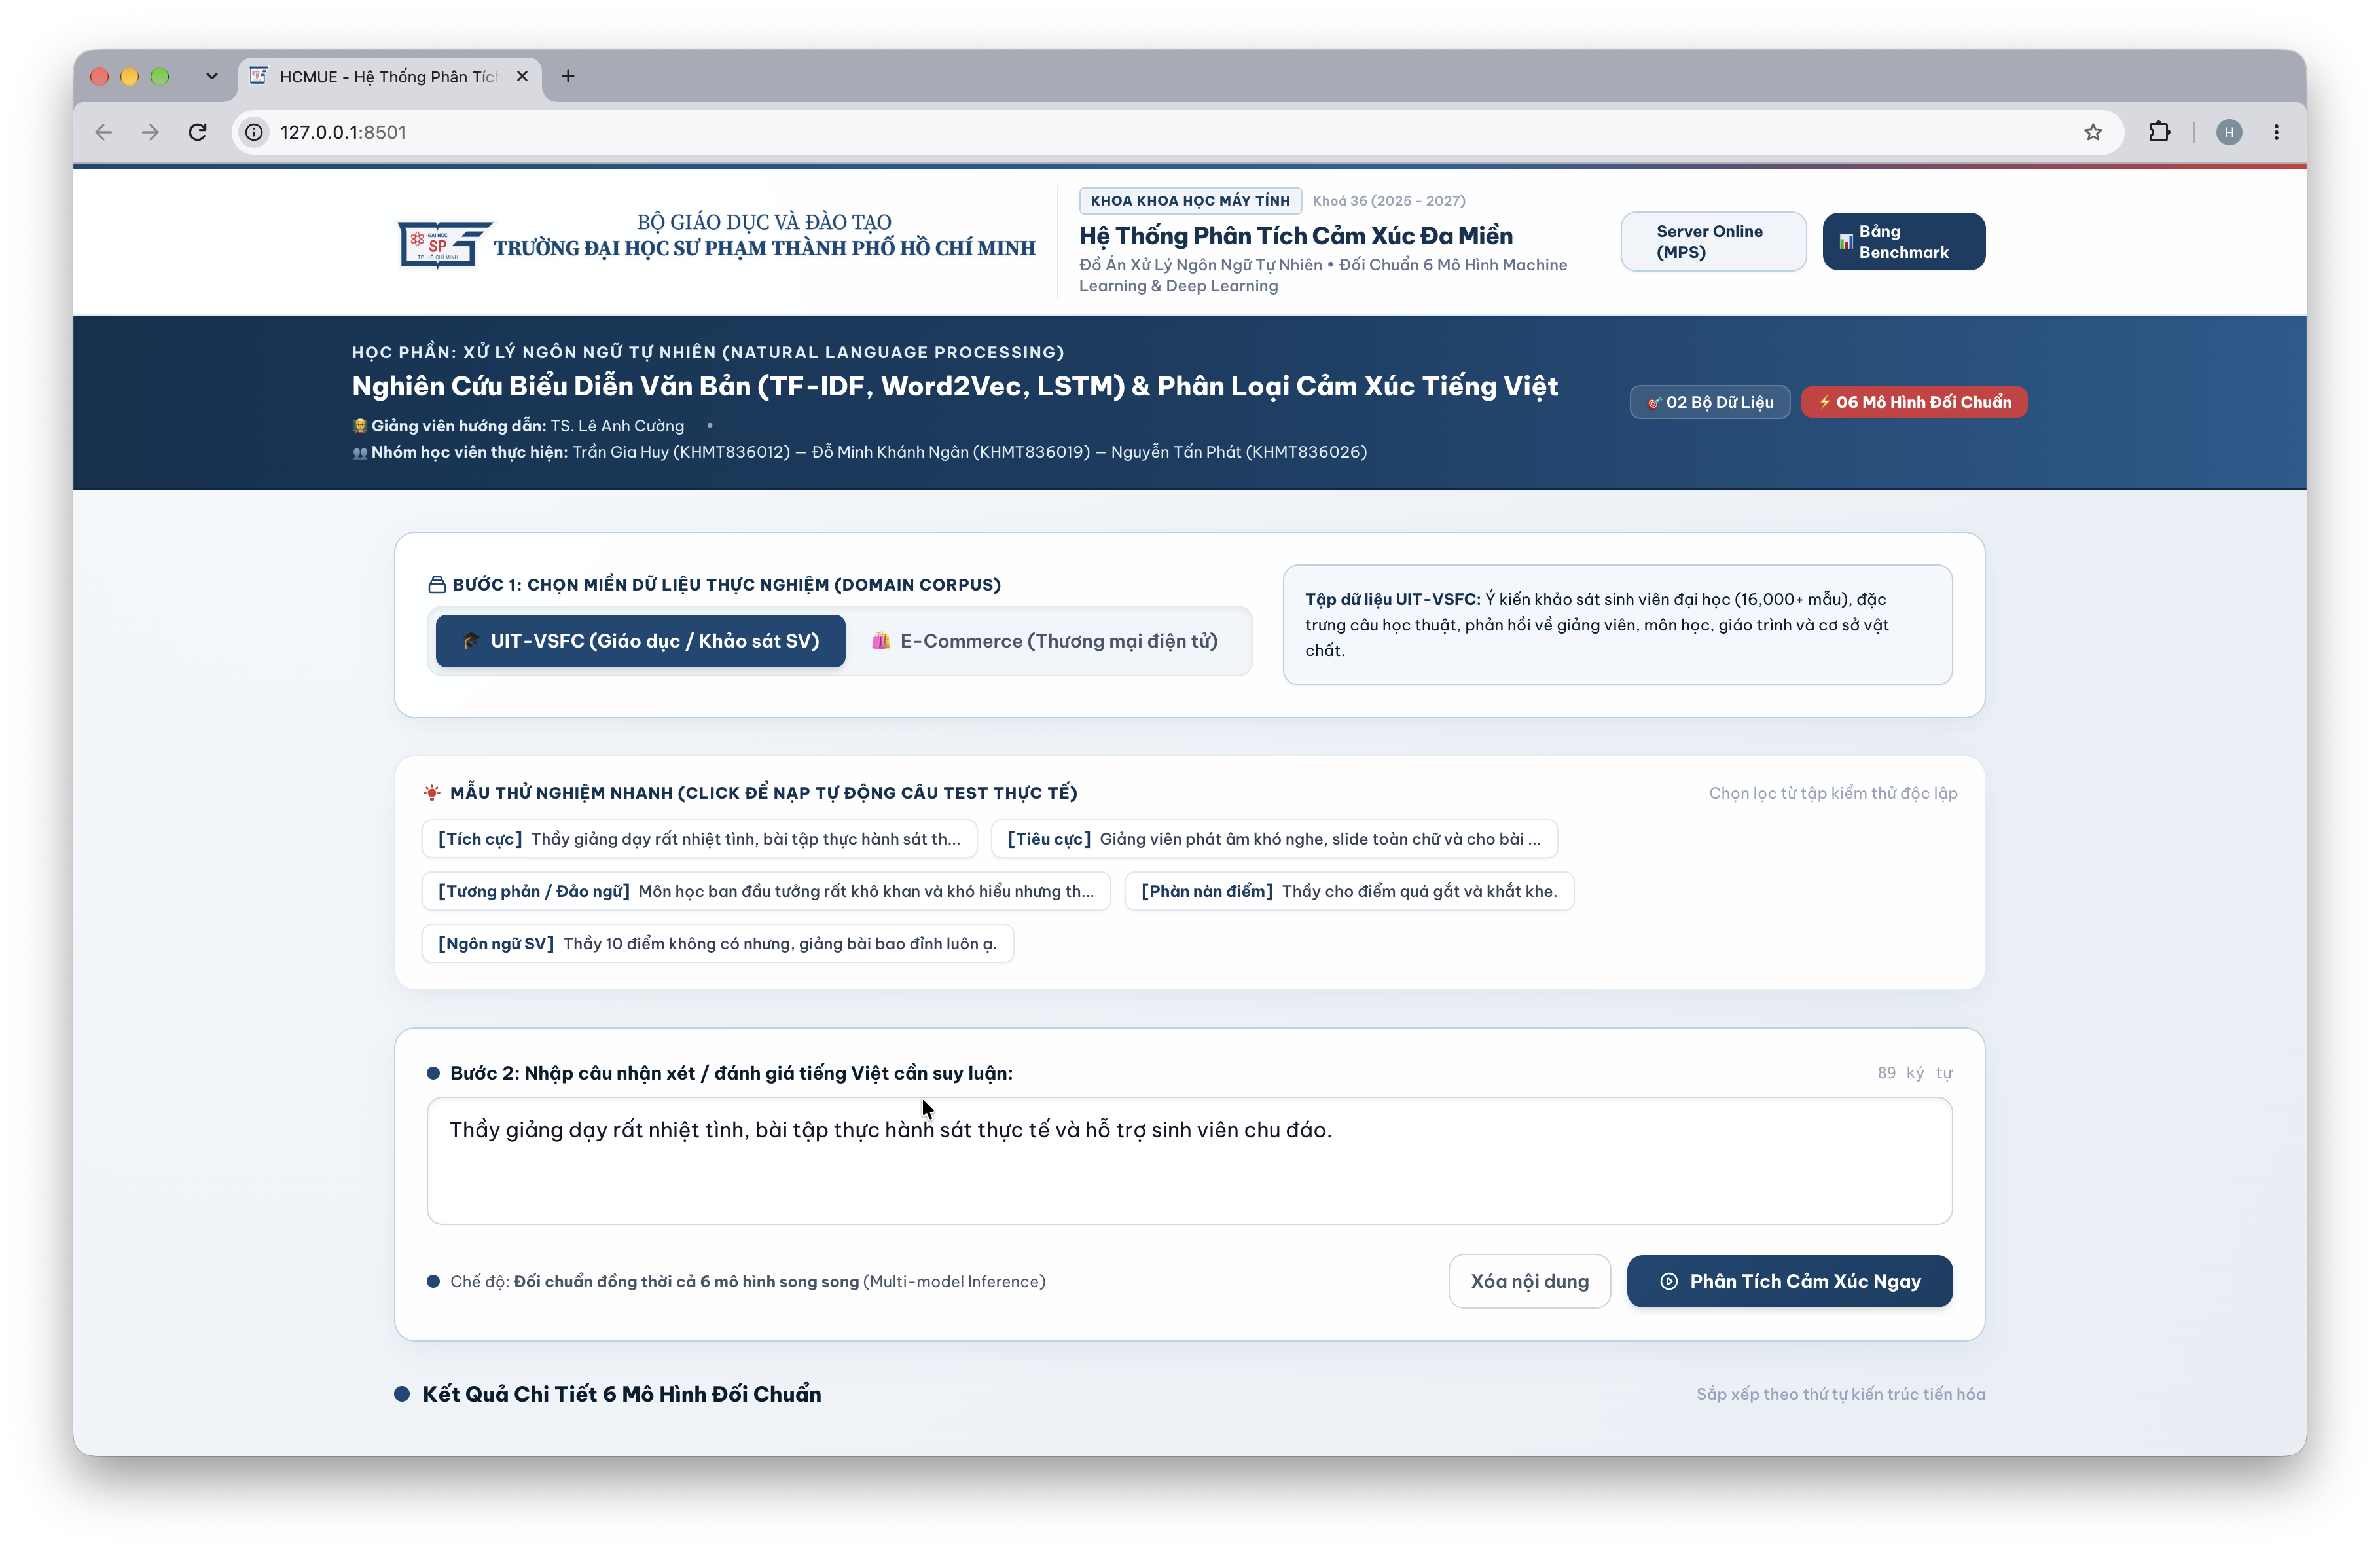
\includegraphics[width=0.92\textwidth]{images/demo_overview.png}
    \caption{Kiến trúc hệ thống và giao diện tổng quan của ứng dụng Demo}
    \label{fig:demo_architecture}
\end{figure}

\subsection{Ý nghĩa thực tiễn của module giải thích quyết định (Explainable AI)}\label{sec:demo_xai}
Điểm khác biệt nổi bật của hệ thống so với một công cụ phân loại cảm xúc thông thường nằm ở module trích xuất và trực quan hóa trọng số Attention theo thời gian thực. Thay vì chỉ trả về một nhãn dự đoán đơn thuần, ứng dụng tô màu trực tiếp lên từng từ trong câu đầu vào theo cường độ trọng số $\alpha_t$ mà mô hình đã học được, cho phép người dùng quan sát ngay lập tức mô hình đang "chú ý" vào cụm từ nào để đưa ra quyết định. Về mặt học thuật, tính năng này hiện thực hóa nguyên lý cốt lõi của lĩnh vực Explainable AI (XAI): biến một quy trình suy luận vốn ẩn (implicit) bên trong hàng triệu tham số mạng nơ-ron thành một bằng chứng tường minh (explicit), có thể kiểm chứng bằng trực giác ngôn ngữ học của con người. Về mặt thực tiễn, đây là yếu tố tiên quyết để một hệ thống phân tích cảm xúc có thể được tin cậy triển khai trong các bối cảnh có tính trách nhiệm giải trình cao, chẳng hạn hỗ trợ giảng viên rà soát phản hồi môn học hoặc bộ phận chăm sóc khách hàng xác minh tự động các đánh giá sản phẩm, thay vì chấp nhận kết quả của mô hình một cách máy móc.

\begin{figure}[H]
    \centering
    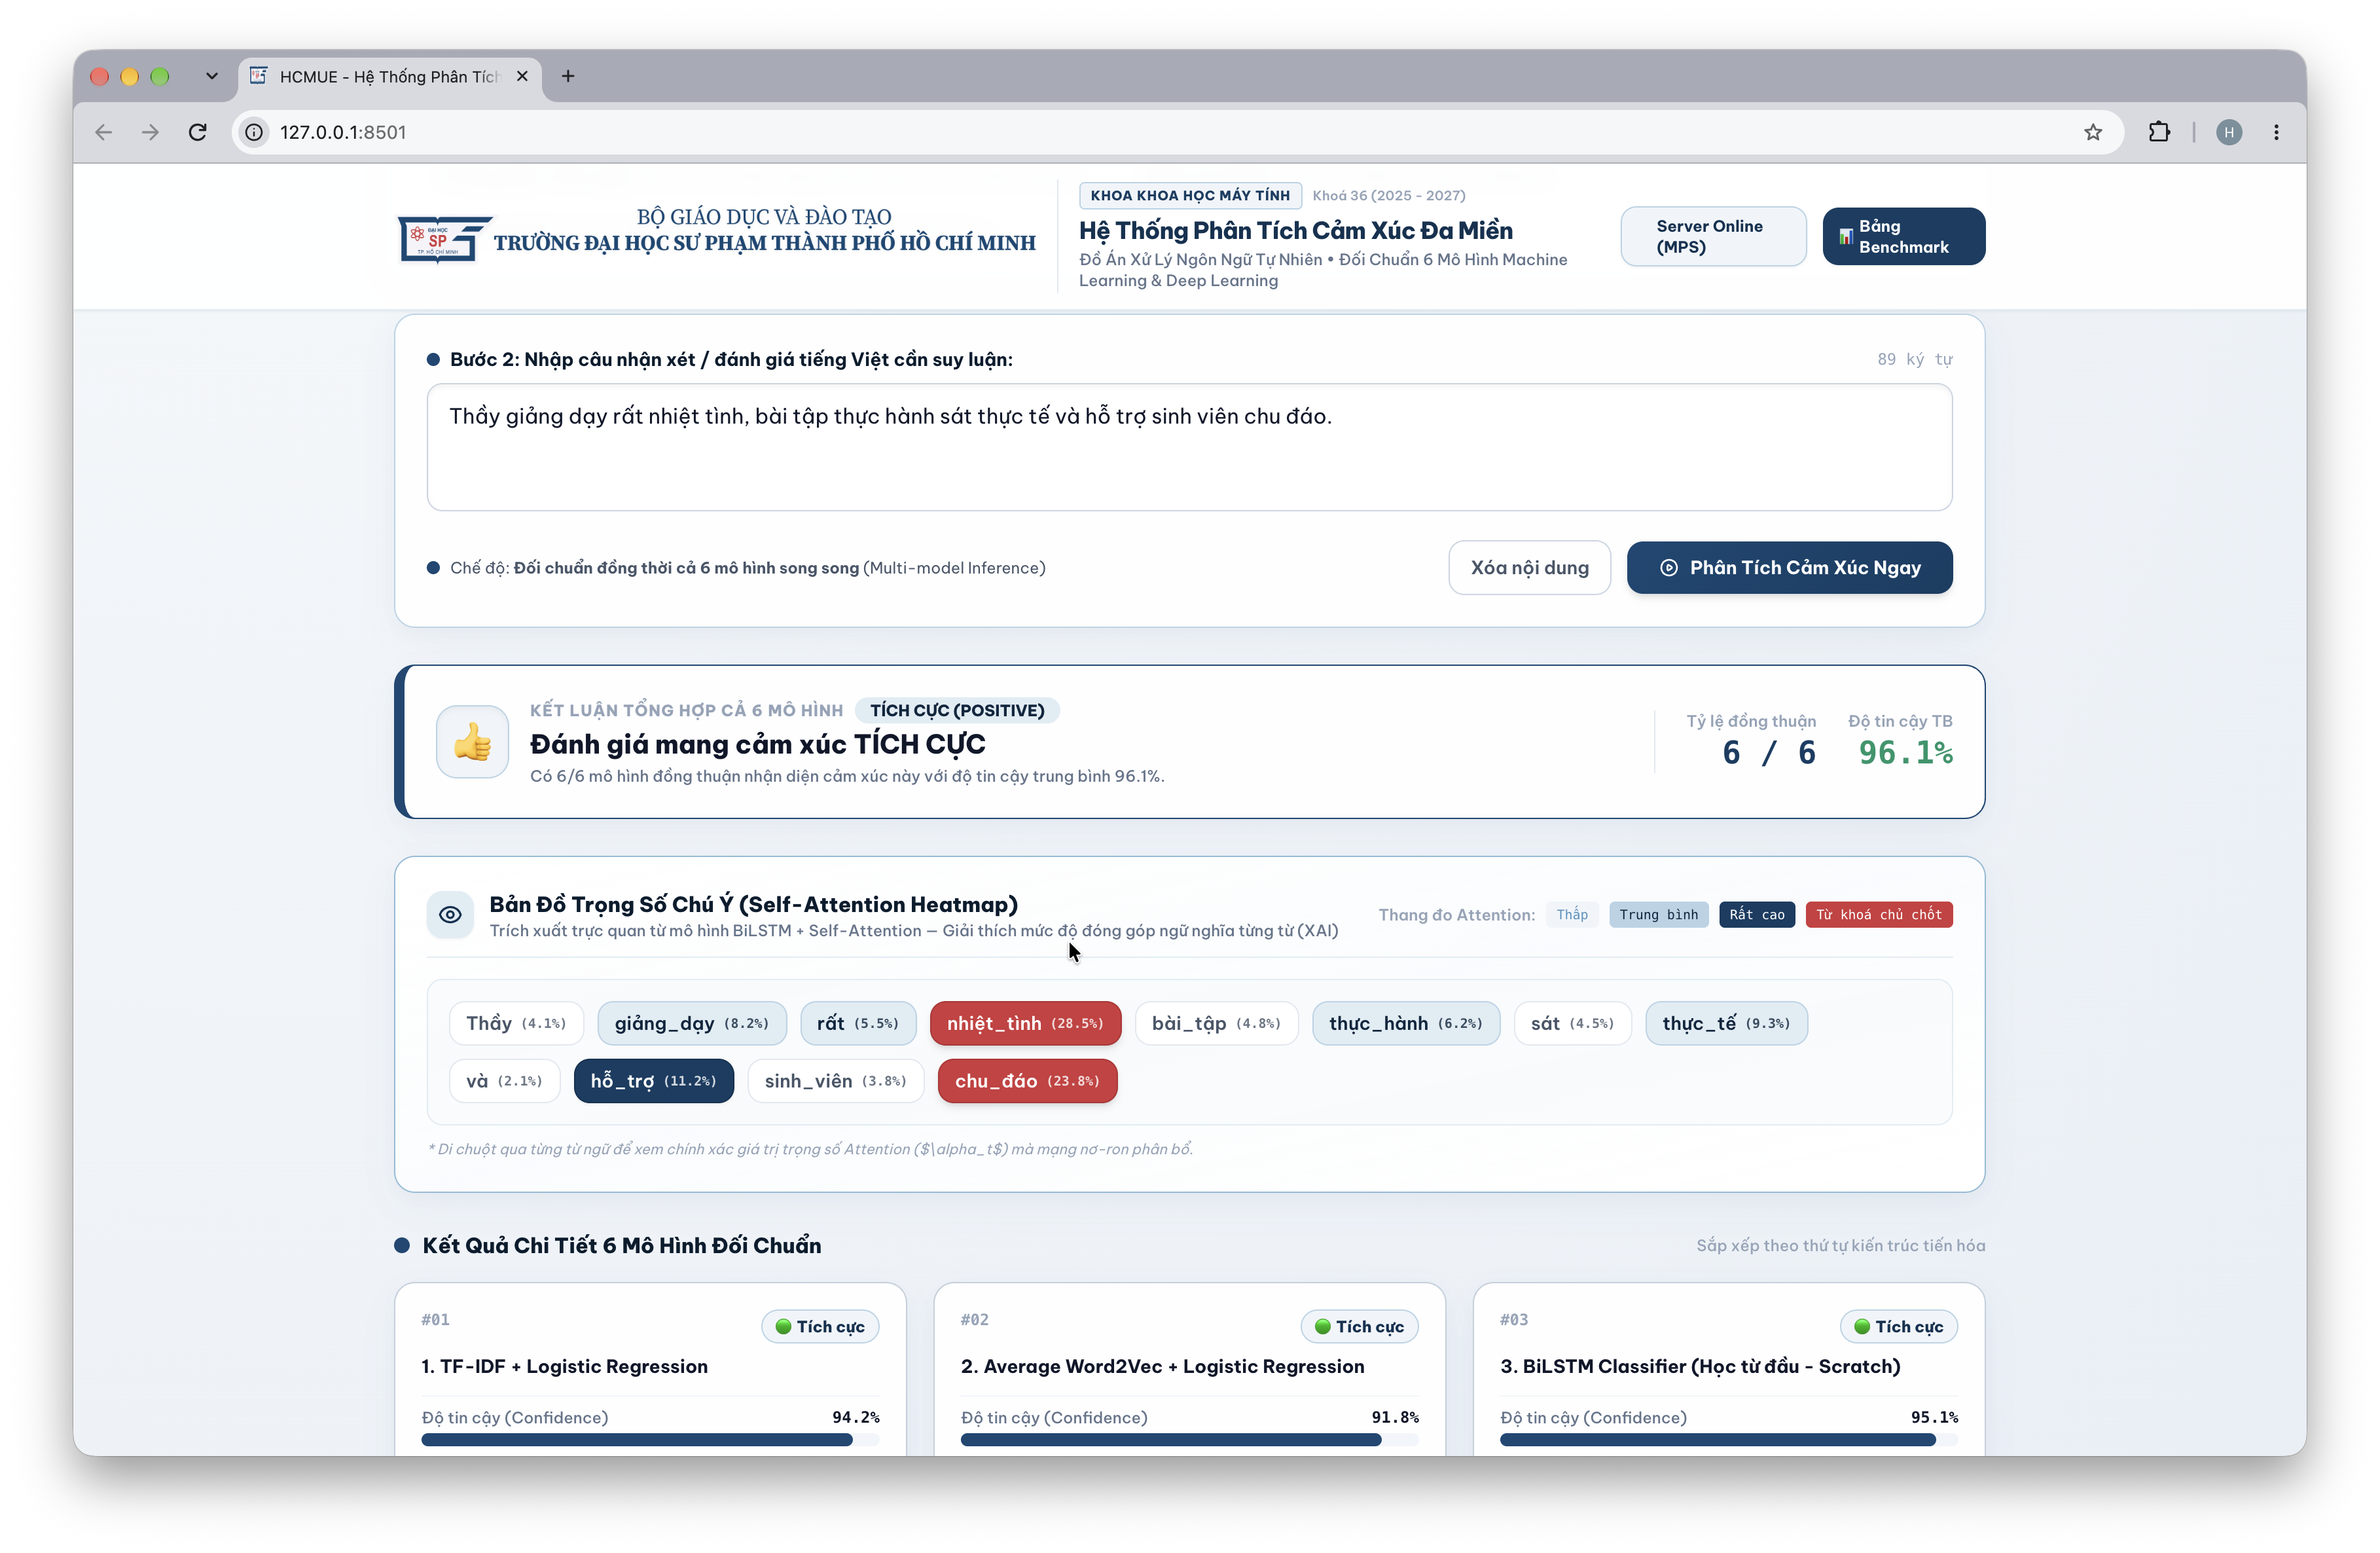
\includegraphics[width=0.92\textwidth]{images/demo_heatmap.png}
    \caption{Bản đồ nhiệt Attention Heatmap minh họa quá trình suy luận thời gian thực}
    \label{fig:demo_heatmap}
\end{figure}

\subsection{Tính khả chuyển và khả năng tái lập (Deployability \& Reproducibility)}\label{sec:demo_deployability}
Nhằm đảm bảo tính khả chuyển của hệ thống trên nhiều môi trường vận hành khác nhau, toàn bộ ứng dụng được đóng gói bằng Docker, tách biệt hoàn toàn phần phụ thuộc (dependencies) của mã nguồn khỏi hệ điều hành máy chủ và loại bỏ hiện tượng xung đột môi trường (``it works on my machine''). Song song đó, một kịch bản khởi chạy tự động (\texttt{run\_app.sh}) được cung cấp nhằm chuẩn hóa quy trình cài đặt, tải checkpoint mô hình và khởi động dịch vụ chỉ bằng một lệnh duy nhất, giúp giảng viên hoặc người đánh giá có thể tái lập (reproduce) toàn bộ kết quả thực nghiệm mà không cần cấu hình thủ công. Ngoài ra, phần giao diện tĩnh (Web SPA) được lưu trữ và phân phối qua GitHub Pages, cho phép truy cập nhanh phần trình bày trực quan của đề tài mà không phụ thuộc vào việc duy trì máy chủ backend liên tục. Việc kết hợp Docker (khả chuyển ở tầng môi trường thực thi), kịch bản triển khai tự động (khả chuyển ở tầng vận hành) và GitHub Pages (khả chuyển ở tầng trình bày) thể hiện tư duy công trình phần mềm (software engineering) đầy đủ, vượt ra ngoài phạm vi một notebook thực nghiệm đơn lẻ, và là minh chứng cho tính sẵn sàng ứng dụng thực tế của kết quả nghiên cứu.

% ------------------------------------------------------------------------------
% CHƯƠNG 5
% ------------------------------------------------------------------------------
\newpage
\section{Kết Luận và Hướng Phát Triển}\label{sec:chuong5}

\subsection{Kết luận}\label{sec:conclusion}
Đề tài đã nghiên cứu chuyên sâu các phương pháp biểu diễn từ và văn bản trong Xử lý ngôn ngữ tự nhiên, tiến hành cài đặt và so sánh đối chuẩn thực nghiệm toàn diện 6 mô hình trên 2 tập dữ liệu thực tế tiếng Việt (\textbf{UIT-VSFC} và \textbf{Vietnamese E-Commerce Reviews}):
\begin{itemize}[leftmargin=1.0cm, itemsep=2pt]
    \item[--] Làm chủ cơ sở lý luận từ biểu diễn rời rạc (One-Hot, TF-IDF), không gian vector dày đặc Word2Vec (CBOW, Skip-Gram, Negative Sampling), mạng nơ-ron hồi quy LSTM hai chiều đến kiến trúc Transformer hiện đại.
    \item[--] Cài đặt thành công mạng \textbf{BiLSTM + Self-Attention} trên PyTorch, chứng minh cơ chế chú ý giúp tăng độ chính xác lên \textbf{91.83\% trên UIT-VSFC} và \textbf{72.50\% trên E-Commerce}, đồng thời cho phép trích xuất Heatmap giải thích trực quan các từ khóa cảm xúc cốt lõi.
    \item[--] Hiện thực hóa thành công mở rộng thực nghiệm trên mô hình Transformer chuyên biệt cho tiếng Việt \textbf{PhoBERT-base-v2} (135M tham số), xác lập kỷ lục vượt trội \textbf{95.50\% trên UIT-VSFC} và \textbf{86.17\% trên E-Commerce} (+15.84\% so với phương pháp truyền thống).
    \item[--] Minh chứng bằng phân tích t-SNE rằng không gian vector chuyển đổi từ dạng rời rạc, phân mảnh của Word2Vec sang cấu trúc phân tách cô đặc, ranh giới rõ rệt của BiLSTM và siêu phẳng phân tách gần như tuyệt đối của PhoBERT Contextual Embeddings.
\end{itemize}

\subsection{Hạn chế của đề tài}\label{sec:limitations}
Bên cạnh những kết quả học thuật và thực nghiệm nổi bật, đề tài vẫn còn một số điểm giới hạn:
\begin{itemize}[leftmargin=1.0cm, itemsep=2pt]
    \item[--] Tài nguyên phần cứng cá nhân chưa cho phép huấn luyện mô hình kích thước lớn (PhoBERT-large hoặc các mô hình LLM từ 7 tỷ tham số trở lên).
    \item[--] Dữ liệu E-Commerce thực tế có mức độ nhiễu cao, nhiều biến thể teencode và các phát biểu mang tính mỉa mai ngầm (sarcasm) đòi hỏi các phương pháp tiền xử lý chuẩn hóa từ vựng tiếng Việt sâu hơn.
\end{itemize}

\subsection{Hướng phát triển trong tương lai}\label{sec:future_work}
Để tiếp tục nâng cao giá trị khoa học và ứng dụng thực tiễn, đề tài đề xuất các hướng nghiên cứu kế tiếp:
\begin{itemize}[leftmargin=1.0cm, itemsep=2pt]
    \item[--] Áp dụng các kỹ thuật tinh chỉnh tham số hiệu quả (\textbf{PEFT / LoRA / QLoRA}) để fine-tune các mô hình nền tảng ngôn ngữ tạo sinh (Generative LLMs như Llama 3, Gemma, PhoGPT) phục vụ phân tích cảm xúc đa khía cạnh (Aspect-Based Sentiment Analysis).
    \item[--] Triển khai hệ thống phân loại cảm xúc thành dịch vụ Web API hoặc bảng điều khiển trực quan tương tác (Interactive Dashboard) phục vụ hỗ trợ phòng đào tạo nhà trường tự động tổng hợp ý kiến sinh viên thời gian thực.
\end{itemize}

% ------------------------------------------------------------------------------
% TÀI LIỆU THAM KHẢO
% ------------------------------------------------------------------------------
\newpage
\phantomsection\label{sec:references}
\begin{center}
    {\large\bfseries TÀI LIỆU THAM KHẢO}
\end{center}
\vspace{0.8cm}

\begingroup
\renewcommand{\section}[2]{}% Bỏ tiêu đề section mặc định của LaTeX
\begin{thebibliography}{99}
\setlength{\itemsep}{6pt}
\sloppy

\bibitem{nguyen2018uit} Kiet Van Nguyen, Vu Duc Nguyen, Phu X. V. Nguyen, Tham T. H. Truong, and Ngan Luu-Thuy Nguyen, “UIT-VSFC: Vietnamese Students’ Feedback Corpus for Sentiment Analysis,” in \textit{Proceedings of the 10th International Conference on Knowledge and Systems Engineering (KSE)}, Ho Chi Minh City, Vietnam, 2018, pp. 19--24. DOI: \href{https://doi.org/10.1109/KSE.2018.8573337}{10.1109/KSE.2018.8573337}.

\bibitem{nguyen2018deep} Phu X. V. Nguyen, Tham T. T. Hong, Kiet Van Nguyen, and Ngan Luu-Thuy Nguyen, “Deep Learning versus Traditional Classifiers on Vietnamese Students’ Feedback Corpus,” in \textit{Proceedings of the 5th NAFOSTED Conference on Information and Computer Science (NICS)}, Ho Chi Minh City, Vietnam, 2018, pp. 1--6. arXiv: \href{https://arxiv.org/abs/1911.07223}{1911.07223}.

\bibitem{mikolov2013efficient} Tomas Mikolov, Kai Chen, Greg Corrado, and Jeffrey Dean, “Efficient Estimation of Word Representations in Vector Space,” in \textit{Proceedings of the International Conference on Learning Representations (ICLR)}, Scottsdale, Arizona, USA, 2013, pp. 1--12. arXiv: \href{https://arxiv.org/abs/1301.3781}{1301.3781}.

\bibitem{mikolov2013distributed} Tomas Mikolov, Ilya Sutskever, Kai Chen, Greg S. Corrado, and Jeffrey Dean, “Distributed Representations of Words and Phrases and their Compositionality,” in \textit{Advances in Neural Information Processing Systems (NeurIPS)}, vol. 26, Lake Tahoe, Nevada, USA, 2013, pp. 3111--3119. arXiv: \href{https://arxiv.org/abs/1310.4546}{1310.4546}.

\bibitem{hochreiter1997lstm} Sepp Hochreiter and Jürgen Schmidhuber, “Long Short-Term Memory,” \textit{Neural Computation}, vol. 9, no. 8, pp. 1735--1780, 1997. DOI: \href{https://doi.org/10.1162/neco.1997.9.8.1735}{10.1162/neco.1997.9.8.1735}.

\bibitem{gers2000learning} Felix A. Gers, Jürgen Schmidhuber, and Fred Cummins, “Learning to Forget: Continual Prediction with LSTM,” \textit{Neural Computation}, vol. 12, no. 10, pp. 2451--2471, 2000. DOI: \href{https://doi.org/10.1162/089976600300015015}{10.1162/089976600300015015}.

\bibitem{goldberg2016primer} Yoav Goldberg, “A Primer on Neural Network Models for Natural Language Processing,” \textit{Journal of Artificial Intelligence Research (JAIR)}, vol. 57, pp. 345--420, 2016. arXiv: \href{https://arxiv.org/abs/1510.00726}{1510.00726}.

\bibitem{jurafsky2026speech} Daniel Jurafsky and James H. Martin, \textit{Speech and Language Processing: An Introduction to Natural Language Processing, Computational Linguistics, and Speech Recognition}, 3rd ed. draft, Stanford University, Aug. 2026. (Chapter 5: Embeddings; Chapter 14: RNNs and LSTMs).

\bibitem{rehurek2010software} Radim Řehůřek and Petr Sojka, “Software Framework for Topic Modelling with Large Corpora,” in \textit{Proceedings of the LREC 2010 Workshop on New Challenges for NLP Frameworks}, Valletta, Malta, 2010, pp. 45--50.

\bibitem{bahdanau2015neural} Dzmitry Bahdanau, Kyunghyun Cho, and Yoshua Bengio, “Neural Machine Translation by Jointly Learning to Align and Translate,” in \textit{Proceedings of the 3rd International Conference on Learning Representations (ICLR)}, San Diego, California, USA, 2015, pp. 1--15. arXiv: \href{https://arxiv.org/abs/1409.0473}{1409.0473}.

\bibitem{vaswani2017attention} Ashish Vaswani, Noam Shazeer, Niki Parmar, Jakob Uszkoreit, Llion Jones, Aidan N. Gomez, Łukasz Kaiser, and Illia Polosukhin, “Attention Is All You Need,” in \textit{Advances in Neural Information Processing Systems (NeurIPS)}, vol. 30, Long Beach, California, USA, 2017, pp. 5998--6008.

\bibitem{nguyen2020phobert} Dat Quoc Nguyen and Anh Tuan Nguyen, “PhoBERT: Pre-trained language models for Vietnamese,” in \textit{Findings of the Association for Computational Linguistics: EMNLP 2020}, 2020, pp. 1037--1042. arXiv: \href{https://arxiv.org/abs/2003.00744}{2003.00744}.

\end{thebibliography}
\endgroup

% ------------------------------------------------------------------------------
% PHỤ LỤC (KHUNG MÃ NGUỒN NHƯ MẪU)
% ------------------------------------------------------------------------------
\newpage
\phantomsection\label{sec:appendix}
\begin{center}
    {\large\bfseries PHỤ LỤC}
\end{center}
\vspace{0.5cm}

\noindent\textbf{1. Mã nguồn mô hình BiLSTM + Self-Attention học biểu diễn văn bản (PyTorch)}
\vspace{0.3cm}

\begin{lstlisting}[language=Python]
import torch
import torch.nn as nn

class SelfAttention(nn.Module):
    """Additive Attention (Bahdanau Style) tinh toan trong so chu y"""
    def __init__(self, hidden_dim, attention_dim=64):
        super().__init__()
        self.projection = nn.Sequential(
            nn.Linear(hidden_dim, attention_dim),
            nn.Tanh()
        )
        self.context_vector = nn.Linear(attention_dim, 1, bias=False)
        
    def forward(self, lstm_out, mask=None):
        u = self.projection(lstm_out)
        scores = self.context_vector(u).squeeze(-1)
        if mask is not None:
            scores = scores.masked_fill(~mask, -1e9)
        weights = torch.softmax(scores, dim=-1)
        doc_vec = torch.bmm(weights.unsqueeze(1), lstm_out).squeeze(1)
        return doc_vec, weights

class BiLSTMAttentionClassifier(nn.Module):
    """Mo hinh BiLSTM ket hop Self-Attention phan loai cam xuc"""
    def __init__(self, vocab_size, emb_dim=100, hidden_dim=128, num_classes=2, pretrained_emb=None):
        super().__init__()
        self.embedding = nn.Embedding(vocab_size, emb_dim, padding_idx=0)
        if pretrained_emb is not None:
            self.embedding.weight.data.copy_(torch.from_numpy(pretrained_emb))
            
        self.lstm = nn.LSTM(emb_dim, hidden_dim, bidirectional=True, batch_first=True)
        self.rep_dim = hidden_dim * 2 # 256
        self.attention = SelfAttention(hidden_dim=self.rep_dim)
        self.classifier = nn.Sequential(
            nn.Dropout(0.3),
            nn.Linear(self.rep_dim, 64),
            nn.ReLU(),
            nn.Dropout(0.3),
            nn.Linear(64, num_classes)
        )
        
    def forward(self, x, lengths=None):
        embed = self.embedding(x)
        lstm_out, _ = self.lstm(embed)
        mask = (x != 0)
        doc_vec, weights = self.attention(lstm_out, mask=mask)
        logits = self.classifier(doc_vec)
        return logits, doc_vec
\end{lstlisting}

\vspace{0.6cm}
\noindent\textbf{2. Mã nguồn Fine-tuning Transformer tiếng Việt PhoBERT}
\vspace{0.3cm}

\begin{lstlisting}[language=Python]
from transformers import AutoTokenizer, AutoModelForSequenceClassification, get_linear_schedule_with_warmup
import torch

def train_phobert_classifier(train_texts, train_labels, val_texts, val_labels, epochs=3, lr=2e-5):
    """Fine-tune vinai/phobert-base-v2 tren tap du lieu cam xuc tieng Viet"""
    tokenizer = AutoTokenizer.from_pretrained("vinai/phobert-base-v2")
    model = AutoModelForSequenceClassification.from_pretrained("vinai/phobert-base-v2", num_labels=2)
    device = torch.device("mps" if torch.backends.mps.is_available() else "cuda")
    model.to(device)
    
    optimizer = torch.optim.AdamW(model.parameters(), lr=lr, eps=1e-8, weight_decay=0.01)
    # Huan luyen qua tung batch va cap nhat tham so
    # ...
    return model, tokenizer
\end{lstlisting}

\end{document}
